\documentclass[a4paper, oneside, 12pt]{book}

% ------------------------------------------------------------------------------
% Setup for table of contents
\setcounter{tocdepth}{3} 	% TOC should label down to subsubsections
\setcounter{secnumdepth}{2}	% TOC should not number further than a subsection number
% ------------------------------------------------------------------------------


% ------------------------------------------------------------------------------
% General Setup
\usepackage[english]{babel}
\usepackage{amsfonts, amsmath, amsthm}		%Formatting symbols, theorems, lemmas, definitions, and examples
\usepackage{eucal}							% Makes the Laplace transform L look a little better

\usepackage{float}							% For making sure tables and figures stay in place
\usepackage{fullpage}						% Create ~1" margins
\usepackage[bottom,flushmargin]{footmisc}	% Put footnotes at bottom of page; don't intent footnotes

\setcounter{chapter}{-1}				% Start with chapter 0

\usepackage{enumitem}					% For custom labels on enumerations
\usepackage{hyperref}					% For inserting links
\usepackage{graphicx} 					% For inserting images
% ------------------------------------------------------------------------------


\usepackage{tikz}
\usetikzlibrary{patterns}
\usetikzlibrary{calc,patterns,decorations.pathmorphing,decorations.markings}

% ------------------------------------------------------------------------------
% Theorems, lemmas, definitions and examples should not be numbered
\newtheorem*{theorem}{Theorem}
\newtheorem*{definition}{Definition}
\newtheorem*{lemma}{Lemma}
\newtheorem*{example}{Example}
% ------------------------------------------------------------------------------

% ------------------------------------------------------------------------------
% Shortcuts
\newcommand{\dd}[2]{\frac{\mathrm{d} #1}{\mathrm{d} #2}}							% d[] / d[]
\newcommand{\pp}[2]{\frac{\partial #1}{\partial #2}}								% partial[] / partial[]

\newcommand{\abs}[1]{\lvert #1 \rvert}												% absolute value

\DeclareMathOperator{\arcsec}{arcsec}												% arc-secant
\DeclareMathOperator{\arccot}{arccot}												% arc-cotangent
\DeclareMathOperator{\arccsc}{arccsc}												% arc-cosecant

\newcommand{\R}{\mathbb{R}}															% Real numbers
\newcommand{\Laplace}[1]{\mathcal{L}\left\{ #1 \right\}\left(s\right)}				% Laplace Transform
\newcommand{\inverseLaplace}[1]{\mathcal{L}^{-1}\left\{ #1 \right\}\left(t\right)}	% Inverse Laplace Transform
% ------------------------------------------------------------------------------


% ------------------------------------------------------------------------------
% Macros for including certain parts of the document. 1 for true, 0 for false.
\def\includeBackgroundReview{1}					% Should the background/review chapter be included?
	\def\includeBackgroundReviewExamples{1}		% Should examples be included in the background/review chapter?
	
\def\includeBasics{1}							% Should the introduction/basics chapter be included?
	\def\includeBasicsExamples{1}				% Should examples be included in the basics chapter?
	
\def\includeFirstOrderLinearODE{1}				% Should the 1st order linear ODE chapter be included?
	\def\includeFirstOrderLinearODEExamples{1}	% Should examples be included in the 1st order linear ODEs chapter?
	
\def\includeHigherOrder{1}						% Should the higher order ODE chapter be included?
	\def\includeHigherOrderExamples{1}			% Should examples be included in the higher order ODE chapter?
	
\def\includeLinearSystems{1}					% Should the linear systems of DiffEq's chapter be included?
	\def\includeLinearSystemsExamples{1}		% Should examples be included in the linear systems chapter?
	
\def\includeLaplaceTransforms{1}				% Should the Laplace transforms chapter be included?
	\def\includeLaplaceTransformExamples{1}		% Should examples be included in the Laplace transforms chapter?

\def\includeAdditionalResources{1}				% Should the additional resources chapter be included?	

% ------------------------------------------------------------------------------


\begin{document}
	% Title page setup
	\title{Intro to Differential Equations: A Summary}
	\author{William Boyles}
	\date{}
		
	\frontmatter
		\maketitle
		\tableofcontents
	
	\mainmatter
		\ifodd\includeBackgroundReview\chapter{Background \& Review}
Everything mentioned in this chapter should already be familiar to you from other math classes.
These topics span two major areas: algebra/pre-calculus and limits.
Ideas from these topics will often be used implicitly or without a passing reference. \\

If you are unfamiliar with anything mentioned, you can use many of the great online resources like Khan Academy to familiarize yourself before moving forward.

\section{Algebra and Pre-Calculus}
\noindent

\subsection{Sets}
\begin{definition}
	A set $A$ is a collection of distinct elements. Those elements can be anything, like numbers, functions, and even other sets.
\end{definition}
We can define a set by giving its elements, like $A = \{-2, 5, 3\}$ or by describing its properties, like $A = \{x \mid x > 0\}$ where the vertical bar means "such that".
If an object $x$ is a member of the set $A$, we write $x\in A$.\bigskip


\noindent
A set $A$ is called a subset of a set $B$ if every element of $A$ is also an element of $B$. 
We can write this as $A \subseteq B$. 
For example, $\{7, 10, 16\} \subseteq \{5, 6, 7, 9, 10, 11, 16\}$. 
Note that this relation can be strict if there exists at least one element in $B$ that is not also an element of $A$. 
Some common sets and their informal definitions are given below:

\begin{table}[H]
	\centering
	\begin{tabular}{c|c|c}
		Set Name & Symbol & Informal Definition                                                                                                                         \\ \hline
		Natural numbers & $\mathbb{N}$ & $\{1, 2, 3, \dots\}$           						                                                                        \\
		Integers & $\mathbb{Z}$ & $\{\dots, -3, -2, -1, 0, 1, 2, 3, \dots\}$                                                                                            \\
		Rational numbers & $\mathbb{Q}$ & $\{\frac{m}{n} \mid m,n \in\mathbb{Z}$ and $n \neq 0\}$                                                                       \\
		Real numbers & $\mathbb{R}$ & Any number on the number line\footnote{Sadly, there is no way to give a stronger formal definition without higher mathematics.}   \\
	\end{tabular}
\end{table}

This means that $\mathbb{N} \subset \mathbb{Z} \subset \mathbb{Q} \subset \mathbb{R}$.\bigskip


\noindent
There are several common operations that can be performed on sets.
The union $A \cup B$ of two sets $A$ and $B$ is the set of all elements that are elements of $A$ or of $B$. 
Similarly, the intersection $A \cap B$ of two sets $A$ and $B$ is the set of all elements that are also elements of both $A$ and $B$.
\begin{example}
	If $A = \{\sqrt{2}, 2, 5, 8\}$ and $B = \{-9, 8, 2.3\}$, what are $A \cup B$ and $A \cap B$?		
\end{example}
To find the union, we combine the sets, making sure to include any repeated element only once:
\begin{equation*}
	A \cup B = \{-9, \sqrt{2}, 2, 2.3, 5, 8\}.
\end{equation*}
Then, since the only element both sets share is 8, we also have
\begin{equation*}
	A \cap B = \{8\}.
\end{equation*}

\subsection{Intervals}
\begin{definition}
	We call a subset $I$ of $\mathbb{R}$ an interval if, for any $a, b \in I$ and $x \in \mathbb{R}$ such that $a \leq x \leq b$, then $x \in I$. 
\end{definition}
We can write an interval more simply using the notation $[a, b]$, which is equivalent to $\{x \in \mathbb{R} \mid a \leq x \leq b\}$. 
This is called a closed interval, and to make the inequalities strict, we can also define an open interval by using parantheses instead of square brackets.\bigskip

In addition, we can mix the two to create half-open intervals, where one inequality is strict and the other isn't. 
For instance, $(2, 5]$ refers to the set $\{x \in \mathbb{R} \mid x < 2 \leq 5\}$
Finally, if the interval is unbounded in either direction, we use the notations $-\infty$ and $\infty$ to indicate that there is no minimum or maximum, respectively.

\begin{example}
	Is $8 \in (-\infty, 4) \cup [8, 100)$?
\end{example}
\begin{answer}
	Since $8 \leq 8 < 100$ is a true statement, $8 \in [8, 100)$. 
	Since we are taking the union with another set, all of the members of the right interval will also be members of the union of intervals. 
	Therefore, the statement is true.
\end{answer}                       % Sets
\subsection{Functions}
\begin{definition}
    A function $f$ is a rule between a pair of sets, denoted $f: D \to C$, that assigns values from the first set, the domain $D$, to the second set, the codomain $C$.
\end{definition}

We call the subset of the codomain $C$ that constitutes all values $f$ can actually attain the range $R \subseteq C$. 
Note that when we draw a graph of a function, all we are doing is drawing all ordered pairs $\{(x, f(x)) \mid x \in D\}$.

\begin{example}
    Find the domain of the following function:
    \begin{equation*}
        f(x) = \frac{1}{(1 - x)\sqrt{5 - x^2}}
    \end{equation*}
\end{example}

\begin{answer}
    We know that $\frac{n}{0}$ is undefined for all $n \in \mathbb{R}$ and $\sqrt{x}$ is only defined for $x \geq 0$. 
    The first condition applies to the first term in the denominator and both conditions apply to the second, giving us
    \begin{equation*}
        (1 - x) \neq 0 \text{ and } 5 - x^2 > 0
    \end{equation*}
    The first condition implies $x \neq 1$ while the second implies $|x| < \sqrt{5}$.
    Putting these together, we find that the domain is
    \begin{equation*}
        \{x \mid x \neq 1, |x| < \sqrt{5}\} \text{ or } (-\sqrt{5}, 1) \cup (1, \sqrt{5})
    \end{equation*}
\end{answer}

We can also compose two functions, such that the ouput of one function is the input of another: 
\begin{equation*}
    (f \circ g)(x) = f(g(x)).
\end{equation*}

\begin{definition}
    A function $g$ is called an inverse function of $f$ if $f(g(x)) = x$ for all x in the domain of g and $g(f(x))$ for all x in the domain of f. 
    We write this as $g = f^{-1}$.
\end{definition}

One common algorithm for finding an inverse function is to set $y = f(x)$, substitute all $x$'s for $y$'s, and then solve for y.
\begin{example}
    Find the inverse function of 
    \begin{equation*}
        f(x) = \frac{5x + 2}{4x - 3}.
    \end{equation*}
\end{example}
\begin{answer}
    We first make the substitutions to set up the algorithm:
    \begin{equation*}
        y = \frac{5x + 2}{4x - 3} \text{ followed by }
        x = \frac{5y + 2}{4y - 3}
    \end{equation*}
    After multiplying both sides by the denominator and simplifying, we have
    \begin{equation*}
        \implies 4xy - 3x = -5y - 2 \\
        \implies y = f^{-1}(x) = \frac{3x - 2}{4x + 5}.
    \end{equation*}
\end{answer}

We say that a function $f$ is even if it satisfies $f(-x) = f(x)$ for all $x \in D$.
Likewise, we say that a function $f$ is odd if it satisfies $f(-x) = -f(x)$ for all $x \in D$. 
Geometrically, we can see that the graph of an even function is symmetric with respect to the $y$-axis, while the graph of an odd function is symmetric with respect to the origin. 

\begin{example}
    Is $f(x) = 2x - x^2$ even, odd, or neither?
\end{example}
\begin{answer}
    \begin{equation*}
        f(-x) = 2(-x) - (-x)^2 = -2x - x^2
    \end{equation*}
    Since $f(-x) \neq f(x)$ and $f(-x) \neq -f(x)$, the function is neither even nor odd.
\end{answer}                   % Functions
\subsection{Complex Numbers}
\begin{definition}
	$i$ is called the imaginary unit. It's defined by $i^2 = -1$.
\end{definition}


\noindent
Complex numbers ($\mathbb{C}$) have the form $z = \alpha + \beta i$, where $\alpha$ and $\beta$ are real numbers. The $\alpha$ part of $z$ is called the real part, so $\Re(z) = \alpha$. The $\beta$ part of $z$ is called the imaginary part, so $\Im(z) = \beta i$.\\

\noindent
Often, complex numbers are visualized as points or vectors in a 2D plane, called the complex plane, where $\alpha$ is the x-component, and $\beta$ is the y-component. Thinking of complex numbers like points helps us define the magnitude of complex numbers and compare them. Since a point $(x,y)$ has a distance $\sqrt{x^2+y^2}$ from the origin, we can say the magnitude of $z$, $\lvert z \rvert$ is $\sqrt{\alpha^2 + \beta^2}$. Thinking of complex numbers like vectors helps us understand adding two complex numbers, since you just add the components like vectors.\\

\noindent
A common operation on complex numbers is the complex conjugate. The complex conjugate of $z = \alpha + \beta i$ is $\overline{z} = \alpha - \beta i$. $z$ and $\overline{z}$ are called a conjugate pair.\\

\noindent
Conjugate pairs have the following properties.
Let $z, w \in \mathbb{C}$.
\begin{align*}
	\overline{z \pm w} &= \overline{z} \pm \overline{w} \\
	\overline{zw} &= \overline{z}\overline{w} \\
	\overline{z} &= z \Leftrightarrow z \in \mathbb{R} \\
	z\overline{z} &= \lvert z \rvert^2 = \lvert \overline{z} \rvert^2 \\
	\overline{\overline{z}} &= z \\
	\overline{z}^n &= \overline{z^n} \\
	z^{-1} &= \frac{\overline{z}}{\lvert z \rvert^2} 
\end{align*}
 			% Complex Numbers
\subsection{Factoring Polynomials}
\noindent
We want to break up a polynomial like $f(x) = a_0 + a_1x^1 + \ldots a_nx^n$ into linear factors so that $f(x) = c(x-b_1)\cdot \ldots \cdot(x - b_n)$. This form makes it simple to see that the roots of $f$, solutions to $f(x) = 0$, are $x = b_1 \ldots b_n$.\\

\noindent
For quadratics, $f(x) = ax^2 + bx + c$, there exists a simple formula that will give us both roots, the quadratic formula
\begin{equation*}
	x = \frac{-b \pm \sqrt{b^2-4ac}}{2a}.
\end{equation*}

\noindent
We can see that when $b^2 - 4ac < 0$, like for $f(x) = x^2 + 5x + 10$, we will get complex roots $\alpha \pm \beta i$. For any polynomial, these roots come in pairs, so if $\alpha + \beta i$ is a root, then so is $\alpha - \beta i$. This means that every conjugate pair $\alpha \pm \beta i$ has a quadratic equation with those roots. Sometimes we will not factor quadratics with complex roots into linear terms.\\

\noindent
Although there do exist explicit formulas for finding roots for cubic (degree 3) and quartic (degree 4) equations, they are too long and not useful enough to memorize. When working by hand, we instead use other tricks to find roots.\\

\noindent
There are a few useful tricks that can help. If the polynomial doesn't have a constant term, then 0 is a root. If all the coefficients sum to 0, then 1 is a root. For certain polynomials with an even number of terms, like all cubics of the form $ax^3 + bx^2 + cax + cb$ we can factor out a term from the first two and last two terms to get $x^2(ax+b)+c(ax+b) = (ax+b)(x^2+c)$. For other polynomials, we might just try guessing and checking values. However, we need a more efficient way that works in general.\\

\noindent
Since we are looking to find linear factors $f(x) = (x-b_1)\cdot \ldots \cdot(x-b_n)$, we can see that the constant term in the polynomial is the product of the roots $b_1 \ldots b_n$. In fact, since the coefficients of polynomials are completely determined by the roots and the leading coefficient, all the coefficients are sums and products of roots. You might remember when factoring quadratics that the coefficient of $x$ term is the sum of the two roots. These rules are called Vieta's formulas.\\

\noindent
So, if we have the constant term, we can check all of its integer factors to see if any are roots. For each root, we can divide, using a technique like synthetic division, to continue finding the rest of the roots. This method is especially useful on tests because the roots tend to be integers.

\input{../common/algebraPreCalc/factoringPolynomials_example.tex} 		% Factoring Polynomials
\subsection{Trig Functions \& The Unit Circle}
\noindent
Imagine aa circle of radius 1 centered at the origin that we'll call the unit circle. The x and y coordinates of a point on the unit circle are completely determined by the angle $\theta$ in radians between the $x$-axis and a line from the origin to the point.\\

\noindent
The function $\cos{\theta}$ tells us x-coordinate of the point, while $\sin{\theta}$ tells us the y-coordinate of the point. The function $\tan{\theta} = \frac{\sin{\theta}}{\cos{\theta}}$ tells us the slope of the line from the origin to the point. Most of the trig functions have geometric interpretations as shown below. The most used ones are $\sin$, $\cos$, $\tan=\frac{\sin}{\cos}$, $\cot = \frac{\cos}{\sin}$, $\csc=\frac{1}{\sin}$, and $\sec=\frac{1}{\cos}$.

\begin{figure}[H]
	\label{unitCircle}
	\centering
	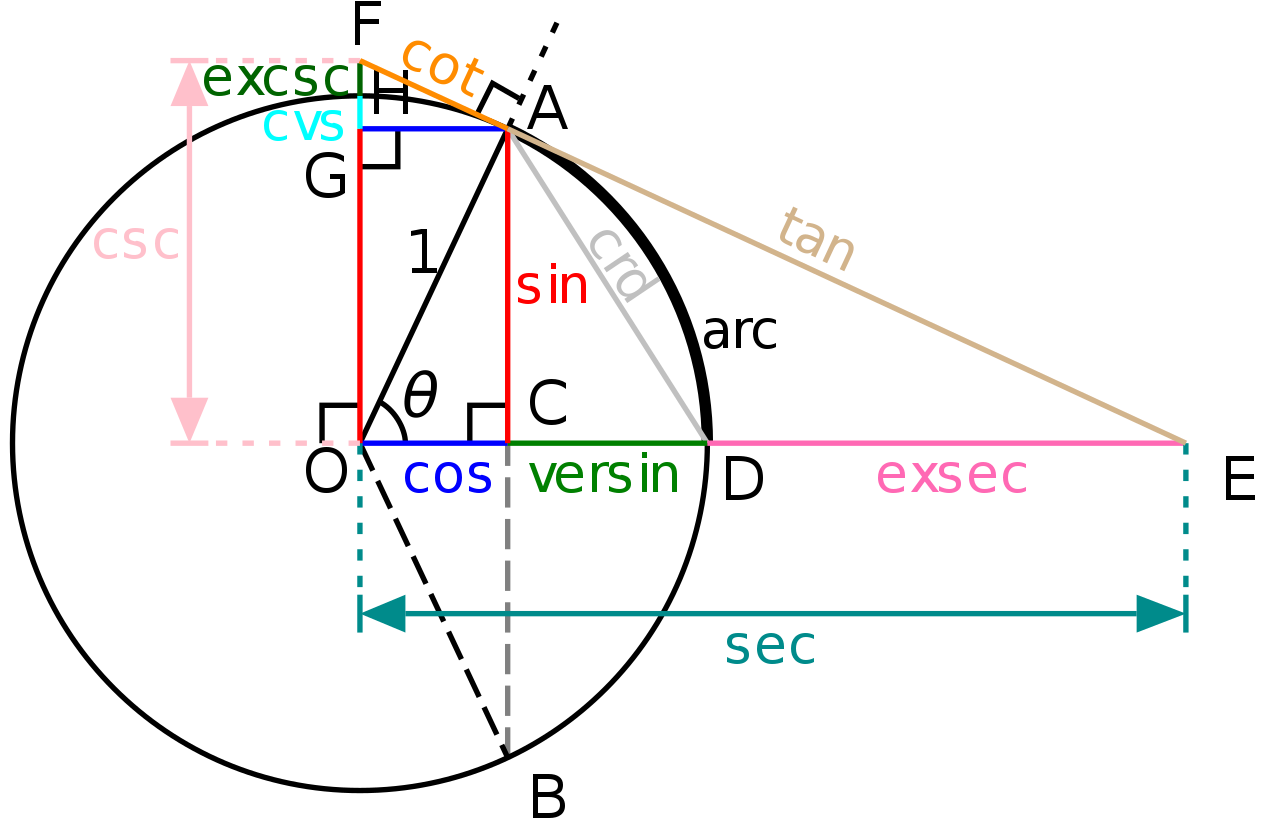
\includegraphics[width = 0.75\textwidth]{../common/algebraPreCalc/unitCircle2.png}
	\caption{\hyperref{https://en.wikipedia.org/wiki/Unit_circle}{}{}{Wikipedia - Unit circle}}
\end{figure}

\noindent
We can also think about the inverses of these trig functions. These are either notated with a -1 exponent on the function, or the prefix arc in front of the function name. Many of these functions are only defined on a part of the domain $\left[0, 2\pi\right]$. Below is a table of the inverse trig functions and their domains.

\begin{table}[H]
	\centering
	\begin{tabular}{l|l}
		Function  & Domain                                                 \\ \hline
		$\arcsin$ & $\left[-1, 1\right]$           						   \\
		$\arccos$ & $\left[-1, 1\right]$                                   \\
		$\arctan$ & $\left(-\infty, \infty\right)$                         \\
		$\arccot$ & $\left(-\infty, \infty\right)$                         \\
		$\arccsc$ & $\left(-\infty, -1\right] \cup \left[1, \infty\right)$ \\
		$\arcsec$ & $\left(-\infty, -1\right] \cup \left[1, \infty\right)$
	\end{tabular}
\end{table}
 	% Trig Functions / Unit Circle
\subsection{Trig Identities}
\noindent
As we could see in Figure \ref{unitCircle}, $\sin$ and $\cos$ form a right triangle with hypotenuse 1. So, using the Pythagorean Theorem,
\begin{equation*}
	\sin^2{\theta} + \cos^2{\theta} = 1.
\end{equation*}
By dividing by $\sin^2$ or $\cos^2$, we can also get
\begin{equation*}
	1 + \cot^2{\theta} = \csc^2{\theta} \text{ and } \tan^2{\theta} + 1 = \sec^2{\theta}.
\end{equation*}
Together, these 3 identities are called the Pythagorean Identities.\\

\noindent
We can also relate functions and co-functions.
\begin{equation*}
	\text{xxx}(\theta) = \text{coxxx}\left(\frac{\pi}{2} - \theta\right).
\end{equation*}

\noindent
Some of the most useful and used identities are the sum and difference.
\begin{align*}
	\sin{\left(\alpha \pm \beta\right)} &= \sin{\alpha}\cos{\beta} \pm \cos{\alpha}\sin{\beta} \\
	\cos{\left(\alpha \pm \beta\right)} &= \cos{\alpha}\cos{\beta} \mp \sin{\alpha}\sin{\beta} \\
	\tan{\left(\alpha \pm \beta\right)} &= \frac{\tan{\alpha} \pm \tan{\beta}}{1 \mp \tan{\alpha}\tan{\beta}} \\
	\sin{\alpha} \pm \sin{\beta} &= 2\sin{\left(\frac{\alpha \pm \beta}{2}\right)}\cos{\left(\frac{\alpha \mp \beta}{2}\right)} \\
	\cos{\alpha} + \cos{\beta} &= 2\cos{\left(\frac{\alpha + \beta}{2}\right)}\cos{\left(\frac{\alpha - \beta}{2}\right)} \\
	\cos{\alpha} - \cos{\beta} &= -2\sin{\left(\frac{\alpha + \beta}{2}\right)}\sin{\left(\frac{\alpha - \beta}{2}\right)} \\
\end{align*} 			    % Trig Identites
\subsection{Exponentials \& Logarithms}
\begin{definition}
	e is the base of the natural logarithm. It's defined by the limit
	\begin{equation*}
		e = \lim\limits_{n\rightarrow\infty}{\left(1+\frac{1}{n}\right)^n}.
	\end{equation*}
\end{definition}
\noindent
$\exp{x} = e^x$ and $\ln{x}$ are inverse functions of each other such that
\begin{equation*}
	e^{\ln{x}} = x \text{ and } \ln{e^x} = x.
\end{equation*}

\noindent
Just like other exponentials, the normal rules for adding, subtracting, and multiplying exponents apply:
\begin{equation*}
	e^xe^y = e^{x+y} \text{, } \frac{e^x}{e^y}=e^{x-y} \text{, and } \left(e^x\right)^k=e^{xk}.
\end{equation*}

\noindent
Similar rules apply for logarithms:
\begin{equation*}
	\ln{x}+\ln{y} = \ln{xy} \text{, } \ln{x}-\ln{y} = \ln{\left(\frac{x}{y}\right)} \text{, and } \ln{\left(a^b\right)} = b\ln{a}.
\end{equation*}

\noindent
We can also write a logarithm of any base using natural logarithms:
\begin{equation*}
	\log_{b}{a} = \frac{\ln{a}}{\ln{b}}.
\end{equation*}

\noindent
$e$ is also unique in that it is the only real number $a$ satisfying the equation
\begin{equation*}
	\frac{\mathrm{d}}{\mathrm{d}x}a^x = a^x,
\end{equation*}
meaning $e^x$ is its own derivative. 		% Exponential and logarithms
\subsection{Partial Fractions}
\noindent
If we have a function of two polynomials $f(x) = \frac{P(x)}{Q(x)}$, it's often easier to break this quotient into a sum of parts where the denominator is a linear or quadratic factor and the numerator is always a smaller degree than the denominator.

\begin{example}
	\begin{equation*}
		\frac{2x-1}{x^3-6x^2+11x-6} = \frac{1/2}{x-1}+\frac{-3}{x-2}+\frac{5/2}{x-3}.
	\end{equation*}
\end{example}

\noindent
One natural way to find these small denominators comes from the linear factors of the denominator where we keep quadratics with complex roots.
This way, when making a common denominator, we get back the original big denominator.
However, there are a few special cases we have to take care of.

\input{../common/algebraPreCalc/linearFactors.tex}
\input{../common/algebraPreCalc/repeatedLinearFactors.tex}
\input{../common/algebraPreCalc/quadraticFactors.tex}
\input{../common/algebraPreCalc/repeatedQuadraticFactors.tex}
\input{../common/algebraPreCalc/improperFractions.tex}
 			% Partial Fractions % Algebra and Pre-Calc\fi 			% Background and Review
		\ifodd\includeBasics\chapter{The Basics of Differential Equations}
\noindent
A differential equation is an equation that relates a function to its derivatives.

% Classifying Differential Equations
\section{Classifying Differential Equations}
\noindent
Below is a list of differential equations
\begin{enumerate}
	\item \begin{equation*}
		t = 7\frac{\mathrm{d}^2 x}{\mathrm{d} t^2} + x\frac{\mathrm{d} x}{\mathrm{d} t}
	\end{equation*}
	\item \begin{equation*}
		\frac{\mathrm{d}y}{\mathrm{d}x} = x^2 + 3xy -7y
	\end{equation*}
	\item \begin{equation*}
		\frac{\partial^2 u}{\partial x^2} + \frac{\partial^2 u}{\partial y^2} = 0
	\end{equation*}
	\item \begin{equation*}
		\frac{\partial^2 y}{\partial t^2} = 4\frac{\partial^2 y}{\partial x^2} + e^{t-x}
	\end{equation*}
	\item \begin{equation*}
		\frac{\mathrm{d} y}{\mathrm{d} x} + 5y = e^x
	\end{equation*}
	\item \begin{equation*}
		\frac{\mathrm{d} y}{\mathrm{d} x} = 3x^2 + y^2
	\end{equation*}
	\item \begin{equation*}
		\frac{\mathrm{d}^2 x}{\mathrm{d} t^2} = \frac{\mathrm{d}x}{\mathrm{d}t} + \cos{x}
	\end{equation*}
	\item \begin{equation*}
		\frac{\mathrm{d}^2 y}{\mathrm{d} x^2} - 2x\frac{\mathrm{d} y}{\mathrm{d} x} + 2y = 0
	\end{equation*}
	\item \begin{equation*}
		\frac{\partial^2 x}{\partial t \partial z} + xt = 5
	\end{equation*}
	\item \begin{equation*}
		\frac{\mathrm{d} x}{\mathrm{d}y} + xy + ty = \ln{y}
	\end{equation*}
\end{enumerate}
Let's think about some of the ways we can classify these equations.
% Order
\subsection{Order}
One way is by this highest order derivative that appears in the equation.
\begin{definition}
	The order of a differential equation is the order of the highest derivative in the equation.
\end{definition}
\noindent
Below is a table of orders and equation numbers.
\begin{table}[H]
	\centering
	\begin{tabular}{c|c}
		Order & Equation Number \\
		\hline
		1 &  2, 5, 6, 10 \\
		2 & 1, 3, 4, 7, 8, 9 \\
	\end{tabular}
\end{table}
% Linearity
\subsection{Linearity}
\noindent
Another useful way to classify differential equations is by linearity.
\begin{definition}
	A differential equation is linear if all terms in the equation involving the dependent varaibles and its derivatives are in linear terms.
\end{definition}
\noindent
"Linear terms" means that dependent varaibles should all be of degree 1, not be multiplied by a derivative involving the same variable, and not be in other functions like $\sin$ or $\ln$. However, this does not exclude differential equations from having parts that are functions of only independent variables, like in equation 4.\\

\noindent
Below is a table of linearity and equation numbers.
\begin{table}[H]
	\centering
	\begin{tabular}{c|c}
		Linearity & Equation Number \\
		\hline
		Linear &  2, 3, 4, 5, 8, 9 \\
		Nonlinear & 1, 6, 7, 10 \\
	\end{tabular}
\end{table}
\noindent
We'll focus a lot of time on linear equations because we have some mathematical tools that are good at dealing with them.
% Ordinary / Partial
\subsection{Ordinary vs. Partial}
\noindent
Another useful classification is by the type. There are two broad types of differential equation: ordinary and partial.
\begin{definition}
	An ordinary differential equation (ODE) is a differential equation where only 1 independent variable involved in the derivatives.
\end{definition}
\begin{definition}
	A partial differential equation (PDE) is a differential equation where 2 or more independent variables are involved in the derivative.
\end{definition}
\noindent
Below is a table of types and equation numbers.
\begin{table}[H]
	\centering
	\begin{tabular}{c|c}
		Type & Equation Number \\
		\hline
		ODE &  1, 2, 5, 6, 7, 8, 10 \\
		PDE & 3, 4, 9 \\
	\end{tabular}
\end{table}
\noindent
We'll work mostly with ODEs.
% Homogeneity
\subsection{Homogeneity}
\begin{definition}
	A differential equation is homogeneous if all terms involve the dependent variable or its derivatives.
\end{definition}

\noindent
Below is a table of homogeneity and equation numbers.
\begin{table}[H]
	\centering
	\begin{tabular}{c|c}
		Homogeneity & Equation Number \\
		\hline
		Homogeneous &  3, 7, 8 \\
		Heterogeneous & 1, 2, 4, 5, 6, 9, 10 \\
	\end{tabular}
\end{table}
\noindent
Homogeneous equations have some nice properties, like always having at least a trivial solution of 0.


\noindent
The three classes of order, linearity, and type are how we describe differential equations in words. Equation 1 would be described as a ``1st order linear ODE''. These definitions also allow us to define explicitly how an nth order linear ODE looks.


\begin{definition}
	An $n$th order linear ODE has the form
	\begin{equation*}
	a_n(x)\frac{\mathrm{d}^n y}{\mathrm{d} x^n} + a_{n-1}(x)\frac{\mathrm{d}^{n-1} y}{\mathrm{d} x^{n-1}} + \ldots + a_0(x)y = b(x).
	\end{equation*}
\end{definition}

% Solutions to DiffEq's
\section{Solutions to Differential Equations}
\begin{definition}
	A solution to an ODE on an interval is a function $f$ that makes the differential equation true on the interval when $f$ is substituted into the equation.
\end{definition}
\noindent
Although this definition seems straightforward it gives us a formal way to check if a function is a solution to a differential equation.

\ifodd\includeBasicsExamples\begin{example}
	Check that $y = t^2\ln{t}$ ($t > 0$) and $y = t^2$  are solutions to the differential equation.
	\begin{equation*}
		t^2y^{\prime\prime} - 3ty^\prime + 4y = 0
	\end{equation*}
\end{example}
\noindent
We'll check $y= t^2\ln{t}$ ($t > 0$) first.
\begin{equation*}
	t^2\left(t^2\ln{t}\right)^{\prime\prime} - 3t\left(t^2\ln{t}\right)^\prime + 4\left(t^2\ln{t}\right) = 0 \text{, } t > 0
\end{equation*}
\begin{equation*}
	t^2\left(3 + 2\ln{t}\right) - 3t\left(t + 2t\ln{t}\right) + 4\left(t^2\ln{t}\right) = 0 \text{, } t > 0
\end{equation*}
\begin{equation*}
	3t^2 + 2t^2\ln{t} - 3t^2 - 6t^2\ln{t} + 4t^2\ln{t} = 0 \text{, } t > 0
\end{equation*}
\begin{equation*}
	0 = 0
\end{equation*}
So $y = t^2\ln{t}$ ($t > 0$) is a solution.\\
Now we'll check $y= t^2$.
\begin{equation*}
	t^2\left(t^2\right)^{\prime\prime} - 3t\left(t^2\right)^\prime + 4\left(t^2\right) = 0
\end{equation*}
\begin{equation*}
	t^2\left(2\right) - 3t\left(2t\right) + 4t^2 = 0
\end{equation*}
\begin{equation*}
	2t^2 - 6t^2 + 4t^2 = 0
\end{equation*}
\begin{equation*}
	0 = 0
\end{equation*}
So $y = t^2$ is also a solution.\fi

% Initial Value Programs
\section{Initial Value Problems}
\noindent
We can see that since solving a differential equation will mean integrating to get rid of derivatives, the $+ C$ from integration will gives us multiple solutions. We call these sets of solutions that differ only in these constants "solution families". If we want to find one specific solution, we need more information about the value of the function and it's derivatives. This type of problem where a differential equation is coupled with function values is called an initial value problem (IVP).\\

\noindent
An initial value problem has the general form.
\begin{equation*}
	\begin{cases}
		a_ny^{(n)} + a_{n-1}y^{(n-1)} + \ldots + a_0y = f(x) \\
		y(x_0) = y_0 \\
		y'(x_1) = y_1 \\
		\vdots \\
		y^{(n)}(x_n) = y_n
	\end{cases}
\end{equation*}
Often, each $x_i$ is 0.

\ifodd\includeBasicsExamples\begin{example}
	The general solution to the IVP
	\begin{equation*}
		\begin{cases}
			y^{\prime\prime} - 5y^\prime + 6y = 0 \\
			y(0) = 3 \\
			y^\prime(0) = 1
		\end{cases}
	\end{equation*}
	is $y = c_1e^{2x} + c_2e^{3x}$. Find the specific solution.
\end{example}
\noindent
Evaluating $y$ at $x = 0$,
\begin{equation*}
	y(0) = c_1 + c_2 = 3
\end{equation*}
Evaluating $y^\prime$ at $x = 0$,
\begin{equation*}
	y^\prime(0) = 2c_1 + 3c_2 = 1
\end{equation*}
To find $c_1$ and $c_2$, we need to solve the system of linear equations
\begin{equation*}
	\begin{cases}
		c_1 + c_2 = 3 \\
		2c_1 + 3c_2 = 1
	\end{cases} \implies \begin{cases}
		c_1 = 8 \\
		c_2 = -5
	\end{cases}
\end{equation*}
So, our specific solution to the IVP is
\begin{equation*}
	y = 8e^{2x} - 5e^{3x}
\end{equation*}\fi

\begin{theorem}[Existence and Uniqueness of Solutions to 1st Order IVPs]
	Consider the IVP
	\begin{equation*}
		\begin{cases}
			\dd{x}{y} = f(x,y) \\
			y(x_0) = y_0
		\end{cases}
	\end{equation*}
	If $f(x,y)$ and $\frac{\partial}{\partial y}f$ are both continuous on some rectangular region containing the point $(x_0, y_0)$, then the IVP has a unique solution $y = y(x)$ on some open interval containing $x_0$.
\end{theorem}

\ifodd\includeBasicsExamples\begin{example}
	Does a solution to the following IVP exist? Is it unique?
	\begin{equation*}
		\begin{cases}
			\dd{y}{x} = x^2 - xy^3 \\
			y(1) = 6
		\end{cases}
	\end{equation*}
\end{example}
\noindent
$f(x,y) = x^2 - xy^3$ and $\frac{\partial f}{\partial y} = -3xy^2$ are continuous on all of $\R^2$. So, the existence and uniqueness theorem tells us that the IVP has a unique solution on an open interval containing $x_0 = 1$.

\begin{example}
	Does a solution to the following IVP exist? Is it unique?
	\begin{equation*}
	\begin{cases}
		\dd{y}{x} = 3y^{2/3} \\
		y(2) = 0
	\end{cases}
	\end{equation*}
\end{example}
\noindent
$f(x,y) = 3y^{2/3}$ is continuous on $y \in \R$, and $\frac{\partial f}{\partial y} = 2y^{-1/3}$ is continuous on $x \in \left(-\infty, 0\right) \cup \left(0, \infty\right)$. Since $\frac{\partial f}{\partial y}$ is not continuous on a domain containing $(2,0)$, the existence and uniqueness theorem does not guarantee a solution.\fi 											% Introduction / Basics	
		\ifodd\includeFirstOrderLinearODE\chapter{1st Order Linear ODE's}
\noindent
1st order linear ODEs are among the simplest differential equations, but learning different techniques to solve them will allow us to develop techniques for solving more complicated types of equations later on.

% Seperable Differential Equations
\section{Separable Differential Equations}
\noindent
The most basic approach for solving a 1st-order differential equation is simply integrating both sides. You're probably already familiar with this technique from taking indefinite integrals. This approach only works when the independent and dependent variables can be arranged on different sides of the equation. We'll formalize this idea with separability.

\begin{definition}
	A 1st order ODE is separable if it can be written in the form
	\begin{equation*}
		\frac{\mathrm{d} y}{\mathrm{d} x} = f(x)g(y)
	\end{equation*}
\end{definition}

\noindent
Separable equations provide a special way of solving them that can be useful. If we treat the derivative like a fraction (which is not formally allowed but OK here),
\begin{equation*}
	\frac{\mathrm{d} y}{\mathrm{d} x} = f(x)g(y) \implies \frac{\mathrm{d} y}{g(y)} = f(x) \mathrm{d}x \implies \int{\frac{\mathrm{d} y}{g(y)}} = \int{f(x) \mathrm{d}x}
\end{equation*}
We then have a function in $y$ on the left and a function in $x$ on the right, meaning we only have to solve for $y$ to get the solution.

\begin{example}
	Solve the following 1st order ODE using separation of variables.
	\begin{equation*}
		\dd{y}{x} = \frac{5}{xy^3}
	\end{equation*}
\end{example}
\noindent
Separating so all terms involving $y$ are on the left,
\begin{equation*}
	y^3 \mathrm{d}y = \frac{5}{x} \mathrm{d}x
\end{equation*}
Integrating,
\begin{equation*}
	\int{y^3 \mathrm{d}y} = \int{\frac{5}{x} \mathrm{d}x} \implies \frac{y^4}{4} = 5\ln{x} + C \implies y = \sqrt[4]{20\ln{x} + C}
\end{equation*}

\begin{example}
	Solve the following IVP using separation of variables.
	\begin{equation*}
		\begin{cases}
			\dd{y}{x} = 2y^2 + xy^2 \\
			y(0) = 1
		\end{cases}
	\end{equation*}
\end{example}
\noindent
Separating,
\begin{equation*}
	\frac{\mathrm{d}y}{y^2} = \left(2 + x\right) \mathrm{d}x \text{, or } y = 0
\end{equation*}
We assume that $y \neq 0$ when dividing, but we need to be careful to include $y = 0$ as a possible solution and check if it satisfies the differential equation and initial conditions.\\

\noindent
Integrating,
\begin{equation*}
	\int{\frac{\mathrm{d}y}{y^2}} = \int{\left(2 + x\right) \mathrm{d}x} \implies \frac{-1}{y} = 2x + \frac{x^2}{2} + C
\end{equation*}
Solving for $y$,
\begin{equation*}
	y = \frac{-2}{x^2 + 4x + C}
\end{equation*}
We ignored $y = 0$, so we need to go back and check if it's a solution to the differential equation.
\begin{equation*}
	0 = 2(0)^2 + x(0)^2
\end{equation*}
Since it's a solution to the differential equation, we'll see if its satisfies the initial conditions of the IVP.
\begin{equation*}
	y(0) = 0 \neq 1 \text{, } y = 0
\end{equation*}
So, $y = 0$ is not a solution to the IVP.\\

\noindent
Solving for $C$ using the initial conditions,
\begin{equation*}
	y(0) = \frac{-2}{(0)^2 + 4(0) + C} = 1 \implies C = -2
\end{equation*}
So,
\begin{equation*}
	y = \frac{-2}{x^2 + 4x -2}
\end{equation*}
is the solution to the IVP.

% Method for solving (Integrating Factor)
\section{Integrating Factor Method}
All 1st order linear differential equations have the form
\begin{equation*}
	a_1(x)\dd{y}{x} + a_0(x)y = b_1(x)
\end{equation*}
which can be rewritten as
\begin{equation*}
	\dd{y}{x} + a(x)y = b(x)
\end{equation*}

\noindent
This equation isn't always separable, and we can't just integrate both sides unless $a_1(x)y$ = 0.\\

\noindent
If $a_0(x) = a_1'(x)$, then we could rewrite the equation and solve by doing the product rule in reverse.
\begin{equation*}
	\left(a_1(x)y\right)' = b_1(x) \implies y = \frac{\int{b_1(x) \mathrm{d}x}}{a_1(x)}
\end{equation*}

\noindent
It's possible to rearrange into this form by multiplying the equation by some function. Specifically, what were looking for is a function $\mu(x)$ such that
\begin{equation*}
	\mu(x)\dd{y}{x} + \mu(x)a(x)y = \mu(x)b(x) \text{ and } \mu'(x) = \mu(x)a(x)
\end{equation*}
This equation involving $\mu(x)$ is one that we know how to solve because it's separable.\footnote{Although we are taking an indefinite integral to find $\mu(x)$, we do not have a $+ C$ term.}
\begin{equation*}
	\mu'(x) = \mu(x)a(x) \implies \mu(x) = e^{\int{a(x) \mathrm{d}x}}
\end{equation*}
Substituting the solution for $\mu(x)$ back,
\begin{equation*}
	e^{\int{a(x) \mathrm{d}x}}\dd{y}{x} + e^{\int{a(x) \mathrm{d}x}}a(x)y = e^{\int{a(x) \mathrm{d}x}}b(x) \implies e^{\int{a(x) \mathrm{d}x}}\dd{y}{x} + \mu'(x)y = e^{\int{a(x) \mathrm{d}x}}b(x)
\end{equation*}
Applying the product rule in reverse,
\begin{equation*}
	y = \frac{\int{\mu(x)} b(x) \mathrm{d}x}{\mu(x)} \text{, } \mu(x) = e^{\int{a(x) \mathrm{d}x}}
\end{equation*}

\begin{example}
	Solve the following 1st order linear ODE.
	\begin{equation*}
		y^\prime - y = 2e^{x}
	\end{equation*}
\end{example}
$a(x) = -1$, so
\begin{equation*}
	\mu(x) = e^{\int{-1 \mathrm{d}x}} = e^{-x}
\end{equation*}
Applying to our equation and solving,
\begin{equation*}
	y^\prime e^{-x} - ye^{-x} = 2 \implies \left(ye^{-x}\right)^\prime = 2 \implies ye^{-x} = 2x + C \implies y = \frac{2x + C}{e^{-x}}
\end{equation*}

% Applications
	% Newton's Law of Cooling
	% Logistic Equation (Viral Spread)
	% Compound Interest
	% RC Circuit\fi 		% 1st order linear ODE's
		\ifodd\includeHigherOrder\chapter{Higher Order Linear ODE's}
\section{Constant Coefficients}
\begin{definition}
	The general form of an nth order linear equation is
	\begin{equation*}
		a_n(x)y^{(n)} + a_{n-1}y^{(n-1)} + \ldots + a_1(x)y' + a_0y = b(x)
	\end{equation*}
	If each $a_i(x)$ is a constant, then the equation has constant coefficients.
\end{definition}

\noindent
We already know how to solve linear first order differential equations using an integrating factor, but let's see if we can develop a method that can solve any order linear, homogeneous differential equation with constant coefficients.

\begin{example}
	Let's try to solve the following equation by guessing and checking likely solutions.
	\begin{equation*}
		y'' - 3y' + 2y = 0
	\end{equation*}
\end{example}
\noindent
Exponentials seem like good guesses. Let's try an exponential of the form $y = Ce^{rx}$ first.
\begin{equation*}
	\left(Ce^{rx}\right)'' - 3\left(Ce^{rx}\right)' + 2\left(Ce^{rx}\right) =  0
\end{equation*}
\begin{equation*}
	Cr^2e^{rx} - 3rCe^{rx} + 2Ce^{rx} = Ce^{rx}\left(r^2 - 3r + 2\right) = 0
\end{equation*}
Since $Ce^{rx} \neq 0$ unless $C = 0$, we only need to solve the quadratic.
Note that the coefficients of the quadratic are the same as the coefficients in the original differential equation.
\begin{equation*}
	r^2 - 3r + 2 = 0 \implies r = 1 \text{, } 2
\end{equation*}
So, our two fundamental solutions are
\begin{equation*}
	\begin{cases}
		y = C_1e^{x} \\
		y = C_2e^{2x}
	\end{cases}.
\end{equation*}
Since these two fundamental solutions are linearly independent, the general solution is the sum of the fundamental solutions.
\begin{equation*}
	y = C_1e^{x} + C_2e^{2x}
\end{equation*}

% Auxillary Equation
\subsection{The Auxiliary Equation}
\noindent
It's not a coincidence that the coefficients of the polynomial that we had to find the 0's of in the above example matched the coefficients of the differential equation. We call this polynomial the auxiliary equation, and it can help us solve linear, homogeneous differential equations with constant coefficients of any order.
\begin{definition}
	A nth order, linear, homogeneous differential equation with constant coefficients has the form
	\begin{equation*}
		a_ny^{(n)} + a_{n-1}y^{(n-1)} + \ldots + a_1y^\prime + a_0y = 0
	\end{equation*}
	The corresponding auxiliary equation is
	\begin{equation*}
		a_nr^n + a_{n-1}r^{n-1} + \ldots + a_1r + a_0 = 0
	\end{equation*}
\end{definition}

\noindent
We now have a method for solving these equations with the roots of the auxiliary equation are all unique. 
\begin{theorem}
	Let $\left\{r_1, \ldots, r_n\right\}$ be the set of unique roots to an auxiliary equation corresponding to a nth order, linear, homogeneous differential equation with constant coefficients. The set of fundamental solutions are $\left\{C_1e^{r_1x}, \ldots, C_ne^{r_nx}\right\}$, and the general solution is
	\begin{equation*}
		y = C_1e^{r_1x} + \ldots + C_ne^{r_nx}
	\end{equation*}
\end{theorem}

\noindent
We can easily extend this method to deal with roots of higher multiplicities.
\begin{theorem}
	Let $\alpha$ be a root with multiplicity $k$ to an auxiliary equation corresponding to a nth order, linear, homogeneous differential equation with constant coefficients. Then $e^{\alpha x}, xe^{\alpha x}, \ldots, x^{k-1}e^{\alpha x}$ are fundamental solutions.
\end{theorem}

\input{./higherOrder/constCoeffs/complexRoots}

% Wronskian
% Application: Mechanical Vibrations (Homogenous, Linear)
	% Simple: mx'' + kx = 0
	% Free Damped: mx'' + by' + ky = 0
% Non-Homogenous Linear DiffEq's
	% Method of Undetermined Coefficients
	% Variation of Parameters
% Forced Vibrations
	% Undamped Forced
		% 1.1 omega != gamma
		% 1.2 omega = gamma
	% Damped Forced\fi 							% Higher (mostly 2nd) Order linear ODE's
		\ifodd\includeLinearSystems\chapter{Linear Systems of Differential Equations}
Although we have a good idea on how to solve many single linear differential equations, it's often useful to think about linear systems of equations, like
\begin{equation*}
	\begin{cases}
		x_1' = 3tx_1 - x_2 + t^2 \\
		x_2' = -x_1 + e^tx_2 - e^{2t}
	\end{cases}
	\to
	\begin{bmatrix}
		x_1 \\ 
		x_2
	\end{bmatrix}' = \begin{bmatrix}
		3t & -1 \\
		-1 & e^t
	\end{bmatrix} \begin{bmatrix}
		x_1 \\
		x_2
	\end{bmatrix} + \begin{bmatrix}
		t^2 \\
		-e^{2t}
	\end{bmatrix}
\end{equation*}
This matrix form, $\vec{x'} = A\vec{x} + \vec{f}$, where $A$ is a square matrix, is called normal form.\\

% Solutions to systems
\section{Solutions to Differential Equations}
\begin{definition}
	A solution to an ODE on an interval is a function $f$ that makes the differential equation true on the interval when $f$ is substituted into the equation.
\end{definition}
\noindent
Although this definition seems straightforward it gives us a formal way to check if a function is a solution to a differential equation.

\ifodd\includeBasicsExamples\begin{example}
	Check that $y = t^2\ln{t}$ ($t > 0$) and $y = t^2$  are solutions to the differential equation.
	\begin{equation*}
		t^2y^{\prime\prime} - 3ty^\prime + 4y = 0
	\end{equation*}
\end{example}
\noindent
We'll check $y= t^2\ln{t}$ ($t > 0$) first.
\begin{equation*}
	t^2\left(t^2\ln{t}\right)^{\prime\prime} - 3t\left(t^2\ln{t}\right)^\prime + 4\left(t^2\ln{t}\right) = 0 \text{, } t > 0
\end{equation*}
\begin{equation*}
	t^2\left(3 + 2\ln{t}\right) - 3t\left(t + 2t\ln{t}\right) + 4\left(t^2\ln{t}\right) = 0 \text{, } t > 0
\end{equation*}
\begin{equation*}
	3t^2 + 2t^2\ln{t} - 3t^2 - 6t^2\ln{t} + 4t^2\ln{t} = 0 \text{, } t > 0
\end{equation*}
\begin{equation*}
	0 = 0
\end{equation*}
So $y = t^2\ln{t}$ ($t > 0$) is a solution.\\
Now we'll check $y= t^2$.
\begin{equation*}
	t^2\left(t^2\right)^{\prime\prime} - 3t\left(t^2\right)^\prime + 4\left(t^2\right) = 0
\end{equation*}
\begin{equation*}
	t^2\left(2\right) - 3t\left(2t\right) + 4t^2 = 0
\end{equation*}
\begin{equation*}
	2t^2 - 6t^2 + 4t^2 = 0
\end{equation*}
\begin{equation*}
	0 = 0
\end{equation*}
So $y = t^2$ is also a solution.\fi
% Homogenous
\section{Homogeneous Systems}
\noindent
Homogeneous systems of linear equations have the form
\begin{equation*}
	\vec{x}^\prime = A\vec{x}
\end{equation*}
We'll see how to find solutions to these types of systems using the eigenvalue method. Finding solutions to these systems will allow us to find homogeneous solutions to heterogeneous systems of equations.

\subsection{Eigenvalue Method}
\noindent
This method allows us to find fundamental solutions using the eigenvalues of the matrix $A$.
Of course, just like with roots of the auxiliary equation, we need to consider the cases of real distinct eigenvalues and eigenvectors, repeated eigenvalues, complex eigenvalues, and defective matrices. 

\input{./linearSystems/homogeneousSystems/realDistinctEigenvalues.tex}
\input{./linearSystems/homogeneousSystems/repeatedEigenvalues.tex}
\input{./linearSystems/homogeneousSystems/defectiveMatrices.tex}
\input{./linearSystems/homogeneousSystems/complexEigenvalues.tex}

% Non-Homogenous
\section{Heterogeneous Systems}
\noindent
Now that we know how to solve the "easy case" of homogeneous systems of linear differential equations, we can tackle the general case of heterogeneous systems. Much like for single equations, we'll look for a homogeneous solution and particular solution, and we'll use undetermined coefficients or variation of parameters to find the particular solution. These methods will then lead into seeing how systems of first order equations relate to single higher order equations.

% Undetermined coefficients
\subsection{Method of Undetermined Coefficients}
\noindent
The rules for undetermined coefficients are very similar for systems and single equations.
Let's say we have a heterogeneous system of the form
\begin{equation*}
	\begin{cases}
		x_1' = a_{11}x_1 + \ldots + a_{1n}x_n + f_1(t) \\
		\vdots \\
		x_n' = a_{n1}x_n + \ldots + a_{nn}x_n + f_n(t).
	\end{cases}.
\end{equation*}
Written in a matrix form,
\begin{equation*}
	\begin{bmatrix}
		x_1' \\
		\vdots \\
		x_n'
	\end{bmatrix} = \begin{bmatrix}
		a_{11} & \ldots & a_{1n} \\
		\vdots & \ddots & \vdots \\
		a_{n1} & \ldots & a_{nn}
	\end{bmatrix} \begin{bmatrix}
		x_1 \\
		\vdots \\
		x_n
	\end{bmatrix} + \begin{bmatrix}
		f_1(t) \\
		\vdots \\
		f_n(t)
	\end{bmatrix},
\end{equation*}
or more compactly as
\begin{equation*}
	\vec{x}' = A\vec{x} + \vec{f}.
\end{equation*}
All we need to do is look at each $f_i(t)$ and write in the $i^{th}$ blank the corresponding guess.
This is like doing undetermined coefficients on each equation in the system.\\

\noindent
This is especially nice when all the $f_i(t)$'s have a similar form because we can write our guess as
\begin{equation*}
	\vec{g}(t) = f_c(t)\vec{v}
\end{equation*}
where $f_c(t)$ is the guess corresponding to $f$ and $\vec{c}$ is a vector of undetermined scalars.

\input{./linearSystems/heterogeneousSystems/undeterminedCoefficients_examples.tex}

% Variation of Parameters
\subsection{Variation of Parameters for Systems}
\noindent
Let $X$ be a fundamental matrix for the homogeneous system.
\begin{equation*}
	\vec{x_h}' = A\vec{x_h}
\end{equation*}
That is,
\begin{equation*}
	\vec{x_h} = X\vec{c}
\end{equation*}
where
\begin{equation*}
	\vec{c} = \begin{bmatrix}
	C_1 \\
	\vdots \\
	C_n
	\end{bmatrix}
\end{equation*}
and the entries of matrix $A$ can be any continuous functions of $t$.

\noindent
We are looking for the particular solution $\vec{x_p}$, to the system
\begin{equation*}
	\vec{x} = A\vec{x} + \vec{f}
\end{equation*}
where $\vec{x_p}$ is of the form
\begin{equation*}
	\vec{x_p} = X\vec{v}
\end{equation*}
where $\vec{v}$ is a vector of functions of $t$ that we'll have to find.

\noindent
Differentiating $\vec{x_p}$,
\begin{equation*}
	\vec{x_p}' = X\vec{v}' + X'\vec{v}
\end{equation*}
From the system we're trying to solve we know that
\begin{equation*}
	X\vec{v}' + X'\vec{v} = A(X\vec{v}) + \vec{f}
\end{equation*}
Since $X' = AX$,
\begin{equation*}
	X\vec{v}' = \vec{f}
\end{equation*}

\noindent
Since the columns of $X$ are always linearly independent, we know that $X^{-1}$ always exists.\\
Multiplying by $X^{-1}$,
\begin{equation*}
	\vec{v}' = X^{-1}\vec{f}
\end{equation*}
Integrating with respect to $t$,
\begin{equation*}
	\vec{v} = \int{X^{-1}\vec{f} \mathrm{d}t}
\end{equation*}
So,
\begin{equation*}
	\vec{x_p} = X\int{X^{-1}\vec{f} \mathrm{d}t}
\end{equation*}
and
\begin{equation*}
	\vec{x} = X\vec{c} + X\int{X^{-1}\vec{f} \mathrm{d}t}
\end{equation*}

\input{./linearSystems/heterogeneousSystems/variationOfParameters_example.tex}
% Higher-order linear diffeq's as systems of 1st order linear diffeq's
\section{Systems and Higher Order Equations}
There is a connection between a system of linear first order equations and a single higher order equation. We'll see how to convert between the two, which will help explain why methods like the auxiliary equation work.

% System to higher order
\subsection{System to Higher Order}
Let's say we have the linear system
\begin{equation*}
	\vec{x}' = A\vec{x} + \vec{f}
\end{equation*}
Writing the system using $x_1, \ldots x_n$ as the components of $\vec{x}$, $f_1, \ldots f_n$ as the components of $\vec{f}$, and $a_{ij}$ as the entry in $A$ on the $i^{th}$ row and $j^{th}$ column,
\begin{equation*}
	\begin{cases}
		x_1' = a_{11}x_1 + \ldots a_{1n}x_n + f_1 \\
		\vdots \\
		x_n' = a_{n1}x_1 + \ldots a_{nn}x_n + f_n
	\end{cases}
\end{equation*}
Let's arbitrarily assign $x_1 = y$. This will allow us to find expressions for $x_2, \ldots x_n$ in terms of $y$ and its derivatives. When we find $x_n$ in these terms and equate $x_n'$ with what's given in the system, we'll have an linear $n^{th}$ order equation.

\ifodd\includeLinearSystemsExamples\input{./linearSystems/systemsAndHigherOrder/systemToHigherOrder_example.tex}\fi

\noindent
The auxiliary polynomial of this higher order equation $p(r)$ and the characteristic polynomial $p(\lambda)$ of the linear system will have exactly the same roots.
% Higher order to system
\subsection{Higher Order to System}
\noindent
Let's say we have the linear, $n^{th}$ order differential equation
\begin{equation*}
	a_ny^{(n)} + \ldots + a_0y = f
\end{equation*}
where $a_0, \ldots a_n$ and $f$ are functions.\\

\noindent
If we let $x_1 = y, x_2 = y', \ldots x_n = y^{(n-1)}$, then we have a system of equations,
\begin{equation*}
	\begin{cases}
		x_1' &= y' = x_2 \\
		\vdots \\
		x_{n-1}' &= y^{(n-1)} = x_n \\
		x_n' &= y^{(n)} = \frac{1}{a_n}\left(f - a_{n-1}x_n - \ldots - a_0x_1\right)
	\end{cases}
\end{equation*}
Rewriting in matrix form,
\begin{equation*}
	\vec{x}' = \begin{bmatrix}
		0 & 1 & 0 & \ldots & 0 \\
		0 & 0 & 1 & \ldots & 0 \\
		\vdots & \vdots	& \vdots & \ddots & \vdots \\
		0 & 0 & 0 & \ldots & 1 \\
		\frac{-a_0}{a_n} & \frac{-a_1}{a_n} & \frac{-a_2}{a_n} & \ldots & \frac{-a_{n-1}}{a_n} 
	\end{bmatrix} \vec{x} + \begin{bmatrix}
		0 \\
		\vdots \\
		0 \\
		\frac{f}{a_n}
	\end{bmatrix}
\end{equation*}
The square matrix has characteristic polynomial $p(\lambda) = \frac{(-1)^{n}}{a_n}\left(a_n\lambda^n + a_{n-1}\lambda^{n-1} + \ldots + a_0\right)$ which has the same zeroes as the the auxiliary equation $a_nr^n + \ldots + a_0$.\\

\noindent
Note that if one starts with a higher order equation, converts it to a system, and the converts the system back to a higher order equation, the result is the original equation. This does not hold true when converting a system to an equation and back to a system. The two solutions will have the same eigenvalues but different eigenvectors.\fi 					% Linear Systems of DiffEq's
		\ifodd\includeLaplaceTransforms\chapter{Laplace Transforms}
\noindent
Laplace transforms allow us to change differential equations into algebraic equations. We can then solve the algebraic equation and ``undo'' the Laplace transform to find the solution to our differential equation.

% Definition
\section{Definition}
\begin{definition}
	Let $f(t)$ be a function that is defined for $t \geq 0$.
	\begin{equation*}
		\Laplace{f} = \int_{0}^{\infty}{e^{-st}f(t) \mathrm{d}t}
	\end{equation*}
	The domain of $F$ is all values of $s$ where the integral is defined and finite.
\end{definition}

\subsection{Linearity}
\noindent
We already know from calculus that the integral is a linear operator.
That is, scalar multiplication can be pulled out of the integral, and the integral of the sum of two functions is the same as the sum of the integrals of the functions.
Since the Laplace transform is just an integral, it is also a linear operator.
So we can say
\begin{equation*}
	\Laplace{cf + g} = c\Laplace{f} + \Laplace{g} \text{, } c \in \R.
\end{equation*}
% Derivations
\section{Derivations}
\noindent
We can use the definition of the Laplace transform and the fact that the Laplace transform is a linear operator to find the Laplace transform of some common functions.

% constant
\subsection{Constant}
Let $a$ be a constant.\\
By definitions of a Laplace transform and an improper integral,
\begin{align*}
	\Laplace{a} &= \lim\limits_{n\to\infty}{\int_{0}^{n}{ae^{-st}\mathrm{d}t}} \\
	&= \frac{a}{s}\lim\limits_{n\to\infty}\left[-e^{-st}\right]_{0}^{n} \text{, } s \neq 0 \\
	&= \frac{a}{s}\lim\limits_{n\to\infty}{\left(1-e^{-sn}\right)} \text{, } s \neq 0 \\
	&= \frac{a}{s} \text{, } s > 0.
\end{align*}
So,
\begin{equation*}
	\Laplace{a} = \frac{a}{s} \text{, } s > 0.
\end{equation*}
% exponential
\subsection{Exponential}
\noindent
Let $a$ be a constant.\\
By definitions of a Laplace transform and an improper integral,
\begin{equation*}
\Laplace{e^{at}} = \lim\limits_{n\to\infty}{\int_{0}^{n}{e^{at}e^{-st}\mathrm{d}t}}
\end{equation*}
\begin{equation*}
 = \lim\limits_{n\to\infty}{\int_{0}^{\infty}{e^{(a-s)t} \mathrm{d}t}}
\end{equation*}
\begin{equation*}
	= \frac{1}{a-s}\lim\limits_{n\to\infty}{\left[e^{(a-s)n}\right]}_{0}^{n} \text{, } s \neq a
\end{equation*}
\begin{equation*}
	= \frac{1}{a-s}\lim\limits_{n\to\infty}{\left(e^{(a-s)n} - 1\right)} \text{, } s \neq a
\end{equation*}
\begin{equation*}
	= \begin{cases}
		\frac{-1}{a-s} & s > a \\
		\text{DNE} & s \leq a
	\end{cases}
\end{equation*}
So,
\begin{equation*}
	\Laplace{e^{at}} = \frac{-1}{a-s} \text{, } s > a
\end{equation*}
% sin and cos
\subsection{Sine and Cosine}

% Sin
\input{./laplaceTransforms/derivations/sin.tex}
% Cos
\input{./laplaceTransforms/derivations/cos.tex}
% nth derivative
\subsection{$n^{th}$ Derivative}
\noindent
We'll use induction to show that
\begin{equation*}
\Laplace{f^{(n)}(t)} = s^n\Laplace{f(t)} - f^{(n-1)}(0) - sf^{(n-2)}(0) - \ldots - s^{n-1}f(0).
\end{equation*}

\noindent
We'll start with the first derivative as a base case. We could use the $0^{th}$ derivative, but this case will give us a little more insight into where the formula comes from.\\
Let $f$ be a differentiable function.
\begin{equation*}
\Laplace{f'(t)} = \lim\limits_{n\to\infty}{\int_{0}^{n}{f'(t)e^{-st}\mathrm{d}t}}
\end{equation*}
Integrating by parts and using the fundamental theorem of calculus,
\begin{equation*}
	 = \left(\lim\limits_{n\to\infty}{\left(f(n)e^{-sn}\right)} - f(0)e^{-s\cdot 0}\right) + \lim\limits_{n\to\infty}{s\int_{0}^{n}{f(t)e^{-st} \mathrm{d}t}}.
\end{equation*}
Assuming that $f(n)$ grows slower than $e^{-sn}$,
\begin{equation*}
	 = \left(0 - f(0)\right) + \lim\limits_{n\to\infty}{s\int_{0}^{n}{f(t)e^{-st} \mathrm{d}t}}.
\end{equation*}
Since the right part of the expression is just $s$ times the definition of $\Laplace{f}$,
\begin{equation*}
	 = s\Laplace{f} - f(0).
\end{equation*}
So,
\begin{equation*}
	\Laplace{f'(t)} = s\Laplace{f} - f(0).
\end{equation*}
Assuming the following is true,
\begin{equation*}
	\Laplace{f^{(n)}(t)} = s^n\Laplace{f(t)} - f^{(n-1)}(0) - sf^{(n-2)}(0) - \ldots - s^{n-1}f(0).
\end{equation*}
We'll show that the $n+1$ case follows.
\begin{equation*}
	\Laplace{f^{(n+1)}(t)} = \Laplace{\left(f^{(n)}\right)'}
\end{equation*}
Using our first derivative formula,
\begin{equation*}
	 = s\Laplace{f^{(n)}(t)} - f^{(n)}(0).
\end{equation*}
Using our general formula,
\begin{align*}
	&= s \left(s^n\Laplace{f(t)} - f^{(n-1)}(0) - sf^{(n-2)}(0) - \ldots - s^{n-1}f(0)\right) - f^{(n)}(0) \\
	&= s^{n+1}\Laplace{f(t)} - f^{(n)}(0) - sf^{(n-1)}(0) s^2f^{(n-2)}(0) - \ldots - s^{n}f(0),
\end{align*}
which is the $n+1$ case, meaning we have proven the general formula as correct.
% polynomial
\subsection{Polynomials}
\noindent
We'll use our derivative formula and induction to show that
\begin{equation*}
	\Laplace{t^n} = \frac{n!}{s^{n+1}} \text{, } n \geq 0.
\end{equation*}
Although the formula for $n = 0$ is clearly the same as $\Laplace{1}$, we'll use $n = 1$ as a base case to get a little more insight into where the formula comes from.\\
\begin{equation*}
	\Laplace{1} = \Laplace{t'} = \frac{1}{s}
\end{equation*}
Using our derivative formula,
\begin{align*}
	\frac{1}{s} &= s\Laplace{t} - 0^{1} \\
	&\implies \Laplace{t} = \frac{1}{s^2}.
\end{align*}
Assuming the following is true,
\begin{equation*}
	\Laplace{t^n} = \frac{n!}{s^{n+1}} \text{, } n \geq 0.
\end{equation*}
We'll show that the $n+1$ case follows.
\begin{equation*}
	\Laplace{t^n} = \Laplace{\left(\frac{t^{n+1}}{n+1}\right)'} = \frac{n!}{s^{n+1}}
\end{equation*}
Using our derivative formula and the linearity of the Laplace transform,
\begin{align*}
	\frac{n!}{s^{n+1}} &= \frac{s}{n+1}\Laplace{t^{n+1}} - 0^{n+1} \\
	&\implies \Laplace{t^{n+1}} = \frac{(n+1)!}{s^{n+2}},
\end{align*}
which is the $n+1$ case, meaning we have proven the general formula as correct.
% translation
\subsection{Translation}
\noindent
Let $a$ be a constant.
\begin{equation*}
	\Laplace{e^{at}f(t)} = \int_{0}^{\infty}{e^{at}f(t)e^{-st} \mathrm{d}t} = \int_{0}^{\infty}{f(t)e^{-(s-a)t} \mathrm{d}t} = \mathcal{L}\left\{f(t)\right\}\left(s-a\right).
\end{equation*}
So,
\begin{equation*}
	\Laplace{e^{at}f(t)} = \mathcal{L}\left\{f(t)\right\}\left(s-a\right).
\end{equation*}
This illustrates how multiplying by $e^{at}$ in the $t$ domain corresponds to a translation by $a$ in the $s$ domain.
% derivative of laplace transforms
\subsection{Derivative of a Laplace Transform}
\noindent
Consider the $n^{th}$ derivative of the Laplace transform of $f$,
\begin{equation*}
	\frac{\mathrm{d}^n}{\mathrm{d}s^n}\left(\Laplace{f(t)}\right) = \frac{\mathrm{d}^n}{\mathrm{d}s^n}\left(\int_{0}^{\infty}{f(t)e^{-st} \mathrm{d}t}\right).
\end{equation*}
We're able to change the order of differentiation and integration here without affecting the result.
\begin{align*}
	&= \int_{0}^{\infty}{f(t)\frac{\mathrm{d}^n}{\mathrm{d}s^n}\left(e^{-st}\right) \mathrm{d}t} \\
	&= \int_{0}^{\infty}{f(t)(-t)^ne^{-st} \mathrm{d}t} \\
	&= (-1)^n\Laplace{t^nf(t)}.
\end{align*}
So,
\begin{equation*}
	\frac{\mathrm{d}^n}{\mathrm{d}s^n}\left(\Laplace{f(t)}\right) = (-1)^n\Laplace{t^nf(t)}.
\end{equation*}
This formula is useful in both directions: finding the derivatives of Laplace transforms, and finding the Laplace transforms of functions multiplied by $t^n$.
% Examples
\ifodd\includeLaplaceTransformExamples\begin{example}
	Find the Laplace transform of $e^{-t}\sin{(3t)}$.
\end{example}
\noindent
Using the translation property,
\begin{equation*}
	\Laplace{e^{-t}\sin{(3t)}} = \mathcal{L}\left\{\sin{(3t)}\right\}(s+1).
\end{equation*}
We from our $\sin$ formula that
\begin{equation*}
	\Laplace{\sin{(3t)}} = \frac{3}{s^2 + 3^2}.
\end{equation*}
So,
\begin{equation*}
	\Laplace{e^{-t}\sin{(3t)}} = \mathcal{L}\left\{\sin{(3t)}\right\}(s+1) = \frac{3}{(s+1)^2 + 3^2}.
\end{equation*}

\begin{example}
	Find the Laplace transform of $t^2(t^2 + 1)(t - 1)(t + 2)$.
\end{example}
\noindent
Using the derivative of the Laplace transform property,
\begin{equation*}
	\Laplace{t^2(t^2 + 1)(t - 1)(t + 2)} = (-1)^2\frac{\mathrm{d}^2}{\mathrm{d}s^2}\Laplace{(t^2 + 1)(t - 1)(t + 2)}.
\end{equation*}
Expanding out the polynomial,
\begin{equation*}
	 = \frac{\mathrm{d}^2}{\mathrm{d}s^2}\Laplace{t^4 + t^3 - t^2 + t - 2}.
\end{equation*}
Using the polynomial formula,
\begin{equation*}
	 = \frac{\mathrm{d}^2}{\mathrm{d}s^2}\left(\frac{4!}{s^5} + \frac{3!}{s^4} - \frac{2!}{s^3} + \frac{1!}{s^2} + \frac{2\cdot 0!}{s^1}\right).
\end{equation*}
Taking the second derivative,
\begin{equation*}
	 \Laplace{t^2(t^2 + 1)(t - 1)(t + 2)} = \frac{6!}{s^7} + \frac{5!}{s^6} - \frac{4!}{s^5} + \frac{3!}{s^4} + \frac{2\cdot 2!}{s^3}.
\end{equation*}

\begin{example}
	Find the Laplace transform of $\left(x^2\right)''$ using the derivative formula. Show it's equal to $\Laplace{2}$.
\end{example}
\noindent
Using the derivative formula,
\begin{equation*}
	\Laplace{\left(x^2\right)''} = s^2\Laplace{x^2} - s\left(x^2\right)'_{x=0} - \left(x^2\right)_{x=0}.
\end{equation*}
Using the polynomial formula,
\begin{equation*}
 	= s^2\frac{2!}{s^3} - 0 - 0.
\end{equation*}
Simplifying,
\begin{equation*}
	\Laplace{\left(x^2\right)''} = \frac{2}{s} = \Laplace{2}.
\end{equation*}

\begin{example}
	Find the Laplace transform of $e^{it}$. Show that it's equal to $\Laplace{\cos{t} + i\sin{t}}$.
\end{example}
Using the exponential formula,
\begin{equation*}
	\Laplace{e^{it}} = \frac{1}{s - i}.
\end{equation*}
Now we'll work on $\cos{t} + i\sin{t}$.
Using the linearity of the Laplace transform,
\begin{equation*}
	\Laplace{\cos{\theta} + i\sin{\theta}} = \Laplace{\cos{t}} + i\Laplace{\sin{t}}.
\end{equation*}
Using the $\sin$ and $\cos$ formulas,
\begin{equation*}
	= \frac{s}{s^2 + 1^2} + i\frac{1}{s^2 + 1^2}.
\end{equation*}
Combining into one fraction,
\begin{equation*}
	= \frac{s+i}{s^2 + 1^2}.
\end{equation*}
Although we normally avoid it, we can factor the denominator into its two complex roots,
\begin{equation*}
	= \frac{s+i}{(s+i)(s-i)}.
\end{equation*}
Canceling out common factors we see that we get the same Laplace transform as we did with $e^{it}$.
\begin{equation*}
	\Laplace{\cos{\theta} + i\sin{\theta}} = \frac{1}{s-i} = \Laplace{e^{it}}.
\end{equation*}
\fi

\noindent
The Laplace transforms of these common functions are summarized in the appendix.
% Inverse Laplace
\section{Inverse Laplace Transforms}
\noindent
Similar to how the derivative is the inverse of the integral, we can think about an inverse Laplace transform that allows us to go back from the $s$ domain to the $t$ domain.
\begin{definition}
	Let $F(s) = \Laplace{f(t)}$. Then $f(t)$ is the inverse Laplace transform of $F(s)$.
	\begin{equation*}
		\inverseLaplace{F(s)} = \inverseLaplace{\Laplace{f(t)}} = f(t)
	\end{equation*}
\end{definition}

\noindent
We don't need to work through the derivations of inverse Laplace transforms because we already did the derivations for Laplace transforms.
% Solving Differential Equations
\section{Solving Equations}
\noindent
Now that we can take the Laplace transform and its inverse of most of the common functions we've seen when solving differential equations, we can use Laplace transforms as another tool to solve differential equations.\\

\noindent
There is a general pattern to how we'll use Laplace transforms to solve differential equations.
\begin{enumerate}[label=\arabic*)]
	\item If needed, arrange the equation into a convenient form in the $t$ domain.
	\item Take the Laplace transform of both sides.
	\item Use algebra, especially partial fraction decomposition and completing the square, to arrange items into a convenient form in the $s$ domain.
	\item Take the inverse Laplace transform of both sides and solve.
\end{enumerate}

% Examples
\ifodd\includeLaplaceTransformExamples\begin{example}
	Solve the following IVP using a Laplace transform.
	\begin{equation*}
		\begin{cases}
			y'' - 2y' - 3y = 0 \\
			y(0) = 1 \\
			y'(0) = 1
		\end{cases}
	\end{equation*}
\end{example}
\noindent
Taking the Laplace transform of both side,
\begin{equation*}
	\Laplace{y'' - 2y' - 3y} = \Laplace{y''} - 2\Laplace{y'} - 3\Laplace{y} = 0
\end{equation*}
\begin{equation*}
	\left(s^2\Laplace{y} - sy'(0) - y(0)\right) - 2\left(s\Laplace{y} - y(0)\right) - 3\left(\Laplace{y}\right) = 0
\end{equation*}
\begin{equation*}
	= \Laplace{y}\left(s^2 - 2s - 3\right) = s - 1
\end{equation*}
Note how the auxiliary equation appears in terms of $s$ here.\\
Solving for $\Laplace{y}$,
\begin{equation*}
	\Laplace{y} = \frac{s - 1}{s^2 - 2s - 3}
\end{equation*}
Rearranging the right side into partial fractions
\begin{equation*}
	\Laplace{y} = \frac{1/2}{s+1} + \frac{1/2}{s-3}
\end{equation*}
Taking the inverse Laplace transform of both sides,
\begin{equation*}
	y = \frac{1}{2}e^{-t} + \frac{1}{2}e^{3t}
\end{equation*}

\begin{example}
	Solve the following IVP using a Laplace transform.
	\begin{equation*}
		\begin{cases}
			y'' + 2y' + 5y = 0 \\
			y(0) = 1 \\
			y'(0) = 5
		\end{cases}
	\end{equation*}
\end{example}
\noindent
Taking the Laplace transform of both sides and solving for $\Laplace{y}$,
\begin{equation*}
	\Laplace{y''} + 2\Laplace{y'} + 5\Laplace{y} = 0
\end{equation*}
\begin{equation*}
	\Laplace{y}\left(s^2 + 2s + 5\right) - y'(0) - sy(0) - 2y(0) = 0
\end{equation*}
\begin{equation*}
	\Laplace{y}\left(s^2 + 2s + 5\right) = s + 7
\end{equation*}
\begin{equation*}
	\Laplace{y} = \frac{s + 7}{s^2 + 2s + 5}
\end{equation*}
The denominator of the right hand side cannot be factored into linear terms. Instead, we'll complete the square.
\begin{equation*}
	= \frac{s + 7}{(s+1)^2 + 2^2}
\end{equation*}
If the numerator was $s+1$, we'd have a $\cos$ that's been shifted left by 1 in the $s$ domain by -1. If the numerator were a multiple of 2, we'd have a $\sin$ that's been similarly shifted. We can rewrite the right hand side as two terms: one for $\cos$ and the other for $\sin$ with the appropriate numerators.
\begin{equation*}
	= \frac{s+1}{(s+1)^2 + 2^2} + 3\frac{2}{(s+1)^2 + 2^2}
\end{equation*}
Taking the inverse Laplace transform of both sides,
\begin{equation*}
	y = e^{-t}\cos{(2t)} + 3e^{-t}\sin{(2t)}
\end{equation*}

\noindent
We can also use the Laplace transform on non-homogeneous equations. The method will even take care of the cases where what would be our guess for the particular solution is already included in the homogeneous solution.
\begin{example}
	Solve the following IVP using a Laplace transform.
	\begin{equation*}
		\begin{cases}
			y'' + 2y' + 5y = e^{-t} \\
			y(0) = 1 \\
			y'(0) = 5
		\end{cases}
	\end{equation*}
\end{example}
\noindent
This equation is the same as the previous example except for the $e^{-t}$, so we can use some of our previous work.
\begin{equation*}
	\Laplace{y}(s^2 + 2s + 5) = s + 7 + \frac{1}{s+1}
\end{equation*}
\begin{equation*}
	 \Laplace{y} = \frac{s^2 + 8s + 8}{(s+1)(s^2 + 2s + 5)}
\end{equation*}
Rearranging the right hand side into partial fractions with completed squares,
\begin{equation*}
	\Laplace{y} = \frac{1}{4}\left(\frac{1}{s+1}\right) + \frac{1}{4}\left(3\frac{s+1}{(s+1)^2 + 2^2} + 9\frac{2}{(s+1)^2 + 2^2}\right)
\end{equation*}
Taking the inverse Laplace transform of both sides,
\begin{equation*}
	y = \frac{1}{4}e^{-t} + \frac{3}{4}e^{-t}\cos{(2t)} + 3e^{-t}\sin{(2t)}
\end{equation*}\fi
% Convolutions
\section{Convolutions}
\subsection{Motivation}
Taking Laplace transforms can be difficult.
We already have some basic formulas derived from linearity properties of integrals that allow us to not evaluate an integral every time.\\

\noindent
One sort of formula that would be nice to have is one relating products of functions.
If we know that
\begin{equation*}
	H(s) = F(s)G(s),
\end{equation*}
where $F$ and $G$ are the Laplace transforms of $f$ and $g$, it'd be nice if we could find the inverse Laplace transform of $H$ to get $h$.
This is one way to define the convolution.

\subsection{Definition \& Convolution Theorem}
\begin{definition}
	Let $F(s)$ and $G(s)$ be the Laplace transforms of functions $f(t)$ and $g(t)$.
	Then
	\begin{equation*}
		F(s)G(s) = \Laplace{f \star g}.
	\end{equation*}
\end{definition}
\noindent
Note how using this definition we can see that $\star$, the convolution operator, is commutative.

\noindent
Defining this function that works like multiplication over Laplace transforms is only really useful if we have a formula for it, so let's derive one.
Starting from the left-hand side of the equation in the definition and applying the integral definition of the Laplace transform,
\begin{equation*}
	F(s)G(s) = \int_{0}^{\infty}{e^{-su}f(u)\d{u}} \cdot \int_{0}^{\infty}{e^{-sv}f(v)\d{v}}.
\end{equation*}
Making this product of integrals into a double integral (we usually do this in reverse when simplifying a double integral),
\begin{equation*}
	= \int_{0}^{\infty}{\int_{0}^{\infty}{e^{-s(u+v)}f(u)g(v)\d{u}}\d{v}}.
\end{equation*}
Letting $t = u+v$,
\begin{equation*}
	= \int_{0}^{\infty}{\int_{0}^{t}{e^{-st}f(u)g(t-u)\d{u}}\d{t}}.
\end{equation*}
Bringing $e^{-st}$ outside of the innermost integral,
\begin{equation*}
	= \int_{0}^{\infty}{e^{-st}\left[\int_{0}^{t}{f(u)g(t-u)\d{u}}\right]\d{t}}.
\end{equation*}
We see that we have the Laplace transform of the expression in the square brackets.
So,
\begin{equation*}
	f \star g = \int_{0}^{t}{f(u)g(t-u)\d{u}}.
\end{equation*}
This is an equivalent way to define the convolution.

\begin{example}
	Compute the convolution of $t^2$ with $t$.
\end{example}
\noindent
Applying the formula we just derived,
\begin{align*}
	t^2 \star t &= \int_{0}^{t}{u^2(t-u)\d{u}} \\
	&= t\frac{u^3}{3} - \frac{u^4}{4} \bigg\rvert_{0}^{t} \\
	&= \frac{t^4}{3} - \frac{t^4}{4} \\
	&= \frac{t^4}{12}.
\end{align*}

\subsection{Properties}
Convolution inherits all the linearity properties of integration.
Let $f(t)$, $g(t)$, and $h(t)$ be piecewise continuous on $[0,\infty)$.
Let $a$ be a real constant.
Then
\begin{enumerate}[label=]
	\item \textbf{Commutativity} -- $f \star = g \star f$
	\item \textbf{Associativity} -- $(f \star g) \star h = f \star (g \star h)$
	\item \textbf{Distributivity over Addition} -- $f \star (g + h) = (f \star g) + (f \star h)$
	\item \textbf{Associativity over Scalar Multiplication} -- $a(f \star g) = (af) \star g$
\end{enumerate}

\subsection{Applications}
When we're using Laplace transforms to solve a differential equation, if we recognize $\Laplace{y}$ as the product of two functions for which we know the inverse Laplace transforms, we can compute a convolution to find $y$.

\begin{example}
	Solve the following differential equation using Laplace transforms and convolutions.
	Let $a$ and $c$ be real constants where $a \neq c$.
	\begin{equation*}
		y' - ay = e^{ct}.\footnotemark
	\end{equation*}
\end{example}
\footnotetext{When we're taking the Laplace transform of both sides, we implicitly use that $y(0)=0$.}
\noindent
Taking the Laplace transform of both sides,
\begin{align*}
	s\Laplace{y} - a\Laplace{y} &= \frac{1}{s-c} \\
	\Laplace{y}(s-a) &= \frac{1}{s-c}.
\end{align*}
Solving for $\Laplace{y}$,
\begin{equation*}
	\Laplace{y} = \frac{1}{s-c} \cdot \frac{1}{s-a}.
\end{equation*}
Recognizing the right-hand side of the equation as the product of the Laplace transforms of $e^{ct}$ and $e^{at}$, we can solve for $y$ by finding the convolution of $e^{ct}$ and $e^{at}$.
Applying our formula,
\begin{align*}
	F(s) = \frac{1}{s-c} &\text{ and } G(s) = \frac{1}{s-a} \\
	f(t) = e^{ct} &\text{ and } g(t) = e^{at}. \\
	y(t) &= f(t) \star g(t) \\
	&= \int_{0}^{t}{e^{cu}e^{a(t-u)}\d{u}} \\
	&= e^{at}\int_{0}^{t}{e^{u(c-a)}\d{u}} \\
	&= e^{at}\left(\frac{e^{(c-a)t}}{c-a} - \frac{1}{c-a}\right) \\
	&= \frac{e^{ct} - e^{at}}{c-a}.
\end{align*}\fi 		% Laplace Transforms
		\ifodd\includeAdditionalResources\chapter{Additional Resources}
% Tests
\section{Tests}
The following are worked free-response questions from three years of AP Calculus BC tests\footnote{These tests questions are owned by the College Board. The questions and College Board's sample responses are available on their website.}.

\subsection{2018 Free-Response Questions}
Questions 1 and 2 are part of the same section and are allotted 30 minutes for completion with the aid of a graphing calculator.
Question 3 through 6 are part of the same section are allotted 1 hour for completion without the aid of a graphing calculator.

\begin{enumerate}
	\item People enter a line for an escalator at  rate modeled by the function $r$ given by
	\begin{equation*}
		r(t) = \begin{cases}
			44\left(\frac{t}{100}\right)^3\left(1-\frac{t}{300}\right)^7 & \text{for } 0 \leq t \leq 300 \\
			0 & \text{for } t > 300,
		\end{cases}
	\end{equation*}
	where $r(t)$ is measured in people per scond and $t$ is measured in seconds.
	As people get on to the escalator, they exit the line at a rate of 0.7 person per second,
	There are 20 people in line at time $t=0$.
	\begin{enumerate}
		\item How many people entered the line for the escalator during the time interval $0 \leq t \leq 300$?
		\item During the time interval $0 \leq t \leq 300$, there are always people in line for the escalator.
			How many people are in line at time $t=300$?
		\item For time $t > 300$, what is the first time $t$ that there are no people in line for the escalator?
		\item For time $0 \leq t \leq 300$, at what time $t$ is the number of people in line at a minimum?
			To the nearest whole number, find the number of people in line at this time.
			Justify your answer.
	\end{enumerate}

	\item Researchers on a boat are investigating plankton cells in a sea.
		At a depth of $h$ meters, the density of plankton cells, in millions of cells per cubic meter, is modeled by $p(h) = 0.2h^2e^{-0.0025h^2}$ for $0 \leq h \leq 30$ and is modeled by $f(h)$ for $h\geq 30$.
		The continuous function $f$ is not explicitly given.
		\begin{enumerate}
			\item Find $p^\prime(25)$.
				Using correct units, interpret the meaning of $p^\prime(25)$ in the context of the problem.
			\item Consider a vertical column of water in this sea with horizontal cross sections of constant area 3 square meters.
				To the nearest million, how many plankton cells are in this column of water between $h=0$ and $h=30$ meters?
			\item There is a function $u$ such that $0 \leq f(h) \leq u(h)$ for all $h \geq 30$ and $\int_{30}^{\infty}{u(h)\d{h}} = 105$.
				The column of water in part (b) is $K$ meters deep, where $K > 30$.
				Write an expression involving one or more integrals that gives the number of plankton cells in the entire column.
				Explain why this number of plankton cells is less than or equal to 2000 million.
			\item The boat is moving on the surface of the sea.
				At time $t \geq 0$, the position of the boat is $(x(t),y(t))$, where $x^\prime(t) = 662\sin{(5t)}$ and $y^\prime(t)=880\cos{(6t)}$.
				Time $t$ is measured in hours, and $x(t)$ and $y(t)$ are measured in meters.
				Find the total distance traveled by the boat over the time interval $0 \leq t \leq 1$.
		\end{enumerate}
	
		\begin{figure}[H]
			\label{2018_3}
			\centering
			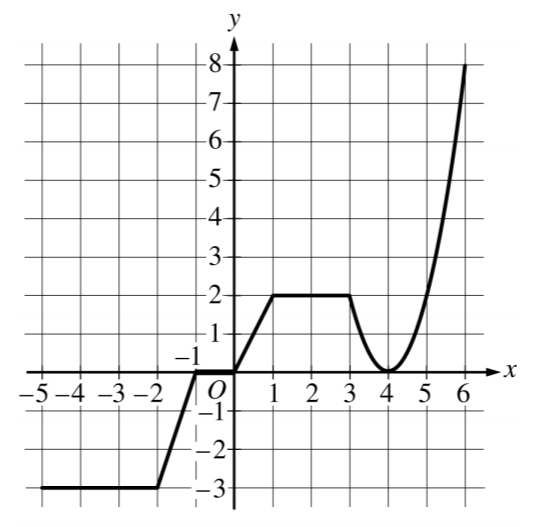
\includegraphics[width=0.5\textwidth]{./additional_materials/2018_3.png}
			\caption{\hyperref{https://apcentral.collegeboard.org/pdf/ap18-frq-calculus-bc.pdf}{}{}{AP Calculus BC 2018 Exam Free-Response Question 3, Graph of $g$}}
		\end{figure}
	
	\item
		The graph of the continuous function $g$, the derivative of a function $f$, is shown above.
		The function $g$ is piecewise linear for $-5 \leq x < 3$ and $g(x)=2(x-4)^2$ for $3 \leq x \leq 6$.
		\begin{enumerate}
			\item If $f(1)=3$, what is the value of $f(-5)$?
			\item Evaluate $\int_{1}^{6}{g(x)\d{x}}$.
			\item For $-5 < x < 6$, on what open intervals, if any, is the graph of $f$ both increasing and concave up?
				Give a reason for your answer.
			\item Find the $x$-coordinate of each point of inflection of the graph of $f$.
				Give a reason for your answer.
		\end{enumerate}
	
		\begin{table}[H]
			\begin{center}
				\begin{tabular}{|c||c|c|c|c|c|}
					\hline
					$t$ (years) & 2 & 3 & 5 & 7 & 10 \\
					\hline
					$H(t)$ (meters) & 1.5 & 2 & 6 & 11 & 15 \\
					\hline
				\end{tabular}
			\end{center}
		\end{table}
	
	\item The height of a tree at time $t$ is given by a twice-differentiable function $H$, where $H(t)$ is measured in meters and $t$ is measured in years.
		Selected values of $H(t)$ are given in the table above.
		\begin{enumerate}
			\item Use the data in the table to estimate $H^\prime(6)$.
				Using correct units, interpret the meaning of $H^\prime(6)$ in the context of the problem.
			\item Explain why there must be at least one time $t$, for $2 \leq t \leq 10$ such that $H^\prime(t) = 2$.
			\item Use a trapezoidal sum with 4 subintervals indicated by the data in the table to approximate the average height of the tree over the time interval $2 \leq 2 \leq 10$.
			\item The height of the tree, in meters, can also be modeled by the function $G$, given by $G(x)=\frac{100x}{1+x}$, where $x$ is the diameter of the base of the tree, in meters.
				When the tree is 50 meters tall, the diameter of the base of the tree is increasing at a rate of 0.03 meters per year.
				According to this model, what is the rate of the change of the height of the tree with respect to time, in meters per year, at the time when the tree is 50 meters tall?
		\end{enumerate}
	
	\begin{figure}[H]
		\label{2018_5}
		\centering
		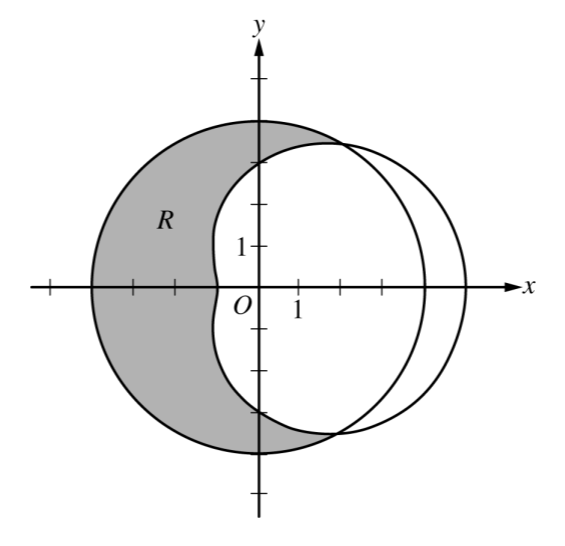
\includegraphics[width=0.5\textwidth]{./additional_materials/2018_5.png}
		\caption{\hyperref{https://apcentral.collegeboard.org/pdf/ap18-frq-calculus-bc.pdf}{}{}{AP Calculus BC 2018 Exam Free-Response Question 5}}
	\end{figure}
	
	\item The graph of the polar curves $r=4$ and $r=3+2\cos{\theta}$ are shown in the figure above.
		The curves intersect at $\theta = \frac{\pi}{3}$ and $\theta = \frac{5\pi}{3}$.
		\begin{enumerate}
			\item Let $R$ be the shaded region inside the graph of $r=4$ and outside the graph of $r=3+2\cos{\theta}$, as shown in the figure above.
				Write an expression involving an integral for the area of $R$.
			\item Find the slope of the line tangent to the graph $r=3+2\cos{\theta}$ at $\theta = \frac{\pi}{2}$.
			\item A particle moves along the portion of the curve  $r=3+2\cos{\theta}$ for $0 < \theta < \frac{\pi}{2}$.
				The particle moves in such a way that the distance between the particle and the origin increases at a constant rate of 3 units per second.
				Find the rate at which the angle $\theta$ changes with respect to time at the instant when the position of the particle corresponds to $\theta = \frac{\pi}{3}$.
				Indicate units of measure.
		\end{enumerate}
	
	\item The Maclaurin series for $\ln{(1+x)}$ is given by
		\begin{equation*}
			x - \frac{x^2}{2} + \frac{x^3}{3} - \frac{x^4}{4} + \ldots + (-1)^{n+1}\frac{x^n}{n} + \ldots .
		\end{equation*}
		On its interval of convergence, this series converges to $\ln{(1+x)}$.
		Let $f$ be a function defined by $f(x) = x\ln{\left(1+\frac{x}{3}\right)}$.
		\begin{enumerate}
			\item Write the first four nonzero erms and the general term of the Maclaurin series for $f$.
			\item Determine the interval of convergence for $f$.
				Show the work that leads to your answer.
			\item Let $P_4(x)$ be the fourth-degree Taylor polynomial for $f$ about $x=0$.
				Use the alternating series estimation bound to find an upper bound for $\abs{P_4(2)-f(2)}$.
		\end{enumerate}
	
\end{enumerate}
\subsection{2018 Free-Response Answers}
\begin{enumerate}
	\item \begin{enumerate}
		\item $r(t)$ tells us the rate at which people enter the line.
			By integrating $r(t)$ over the given interval, we can find the total number of people who entered the line.
			Using a calculator,
			\begin{equation*}
				\int_{0}^{300}{r(t)\d{t}} = \int_{0}^{300}{44\left(\frac{t}{100}\right)^3\left(1-\frac{t}{300}\right)^7\d{t}} = 270 \text{ people}.
			\end{equation*}
		\item We know that at $t=0$, there are already 20 people in line.
			Combining this fact with our answer from part (a), we know that $270+20=290$ people entered the line in the time interval.
			We also know that people leave the line at a constant rate of 0.7 people per second.
			Integrating this rate over the time interval will give us the number of people who left the line.
			\begin{equation*}
				\int_{0}^{300}{0.7\d{t}} = 210 \text{ people}.
			\end{equation*}
			So, there are $290-210=80$ people in line at $t=30$.
		\item We know from our answer in (b) that there are 80 people in line at $t=300$.
			We see from $r(t)$ that no more people are entering the line when $t>300$.
			So, the only thing that contributes to changing the number of people in line is people constantly leaving at a rate of 0.7 people per second.
			\begin{equation*}
				300\text{s} + \frac{80 \text{ people}}{0.7\text{ people/s}} \approx 414.286\text{s}.
			\end{equation*}
		\item Combining the fact that there are initially 20 people in line, the inflow rate is given by $r(t)$ and the outflow rate is 0.7, we can get that the number of people in line at time $x$ is modeled by
		\begin{equation*}
			20 + \int_{0}^{x}{\left(r(t)-0.7\right)\d{t}}.
		\end{equation*}
		Finding when the derivative is 0,
		\begin{equation*}
			r(t) - 0.7 = 0 \implies t = 33.013 \text{ or } 166.575.
		\end{equation*}
		Finding the number of people in line at these times and the endpoints 0 and 300,
		\begin{align*}
			\text{people}_{0} &= 20 \\
			\text{people}_{33.013} &= 3.803 \\
			\text{people}_{166.575} &= 158.070 \\
			\text{people}_{300} &= 80,
		\end{align*}
		we see that the fewest number of people occurs when $t\approx 33.013\text{s}$.
	\end{enumerate}

	\item \begin{enumerate}
		\item Using a calculator, we see that $p^\prime(25) = -1.17906$.
			In the context of the problem, this value means that at a depth of 25 meters, the density of plankton is decreasing at a rate of 1.17906 million plankton per cubic meter per meter.
		\item The vertical density of the plankton in the column is given by $p(h)*3\text{m}^2$.
			Integrating this density function for $0 \leq h \leq 30\text{m}$, we'll get the total number of plankton on the column.
			\begin{equation*}
				\int_{0}^{30}{3p(h)\d{h}} \approx 1675.414.
			\end{equation*}
			So, there are 1675.414 million plankton in the column from 0 to 30 meters depth.
		\item The total number of plankton in the entire vertical column with cross section area $A\text{m}^2$ is given by
			\begin{equation*}
				P = \int_{0}^{\infty}{A\text{density}(h)\d{h}}.
			\end{equation*}
			We can break this integral up, and we can use $A=3\text{m}^2$ for our particular column.
			\begin{equation*}
				P = 3\int_{0}^{30}{p(h)\d{h}} + 3\int_{30}^{\infty}{f(h)\d{h}}.
			\end{equation*}
			Since $u(h) \geq f(h)$ for $h \geq 30$, we can write the following inequality, the right side of which we can numerically evaluate:
			\begin{align*}
				P &\leq 3\int_{0}^{30}{p(h)\d{h}} + 3\int_{0}^{\infty}{u(h)\d{h}} \\
				&\leq 1675.414 + 3(105) \\
				&\leq 1990.414.
			\end{align*}
			So, we see that the number of plankton in the entire vertical column is at most 1990.414 million, which is strictly less than 2000 million.
		\item Since the position of the boat is parametric, we can use the parametric arc length formula to find the total distance traveled for $0 \leq t \leq 1\text{hr}$.
			\begin{align*}
				D &= \int_{0}^{1}{\sqrt{(x^\prime(t))^2+(y^\prime(t))^2}\d{t}} \\
				&= \int_{0}^{1}{\sqrt{\left(662\sin{(5t)}\right)^2 + \left(880\cos{(6t)}\right)^2}\d{t}} \\
				&\approx 757.456.
			\end{align*}
			So, for $0 \leq t \leq 1\text{hr}$, the boat travels a distance of 757.456 meters.
	\end{enumerate}

	\item \begin{enumerate}
		\item Trying to treat this like an initial value problem would be too tedious with all the piecewise parts of $g$.
			Plus, it would be doing more than the question asked because it only wants the value of $f$ at a particular point, not an expression for $f$.
			Instead, we can use the fact that $g$ is the derivative of $f$ and apply the Fundamental Theorem of Calculus.
			\begin{equation*}
				\int_{-5}^{1}{g(x)\d{x}} = f(1) - f(-5) = 3 - f(-5).
			\end{equation*}
			Evaluating the integral geometrically,
			\begin{equation*}
				\int_{-5}^{1}{g(x)\d{x}} = -(9+\frac{3}{2}) + 1 = \frac{-19}{2}.
			\end{equation*}
			Solving for $f(-5)$,
			\begin{equation*}
				\frac{-19}{2} = 3 - f(-5) \implies f(-5) = \frac{25}{2}.
			\end{equation*}
		\item Evaluating the integral,
			\begin{align*}
				\int_{1}^{6}{g(x)\d{x}} &= \int_{1}^{3}{2\d{x}} + \int_{3}^{6}{2(x-4)^2\d{x}} \\
				&= 2x\biggr\rvert_{1}^{3} + \frac{2}{3}(x-4)^3\biggr\rvert_{3}^{6} \\
				&= 4 + \frac{18}{3} \\
				&= 10.
			\end{align*}
		\item $f$ is increasing when its first derivative is positive and concave up when its second derivative is positive.
			Since $g$ is the derivative of $f$, we can also say that $f$ is increasing when $g$ is positive and concave up when $g$ is increasing.
			$g$ is positive on $(0,4) \cup (4,6]$.
			$g$ is increasing on $(-2,-1) \cup (0,1) \cup (4,6)$.
			Taking the intersection of these intervals, we see that $f$ is increasing and concave up on $(0,1) \cup (4,6)$.
		\item $f$ has an inflection point when its second derivative is equal to 0, changing sign.
			Since $g$ is the derivative of $f$, we can also say that $f$ has an inflection point when the derivative of $g$ is equal to 0, changing sign.
			Although we see by looking at the graph that the derivative of $g$ is 0 over several intervals, it does not change sign.
			The only place the derivative is 0 and changes sign is at $x=4$.
	\end{enumerate}

	\item \begin{enumerate}
		\item We can approximate $H^\prime(6)$ as the average rate of change between $t=5$ and $t=7$.
			\begin{equation*}
				H^\prime(6) \approx \frac{H(7)-H(5)}{7-5} = \frac{11-6}{7-5} = \frac{5}{2}.
			\end{equation*}
			In the context of this problem $H^\prime(6) \approx = \frac{5}{2}$ means that at 6 years, the tree is growing at a rate of 5/2 meters per year.
		\item Looking at the average rate of change between $t=3$ and $t=5$,
			\begin{equation*}
				\bar{H^\prime}_{3,5} = \frac{H(5)-H(3)}{5-3} = \frac{6-2}{5-3} = 2.
			\end{equation*}
			Since $H$ is differentiable, it is also continuous.
			So, by the mean value theorem, there is at least one point $3 \leq c \leq 5$ (which is a sub-interval of $2 \leq t \leq 10$) such that $H^\prime(c) = 2$. 
		\item We know that the average value of a continous function $f$ over some interval $[a,b]$ is
			\begin{equation*}
				\bar{f}_{a,b} = \frac{1}{b-a}\int_{a}^{b}{f(x)\d{x}}.
			\end{equation*}
			So, over our interval of $[2,10]$, we need to approximate this integral using trapezoids.
			Because the sub-interval widths given by the table are not equally-sized, we can't apply the shortcut trapezoidal rule.
			However, we can still approximate the area using trapezoids.
			\begin{equation*}
				\frac{1}{10-2}\int_{2}^{10}{H(x)\d{x}} \approx \frac{1}{8}\left(\frac{1.5+2}{2}1+\frac{2+6}{2}2+\frac{6+11}{2}2+\frac{11+15}{2}3\right) = \frac{1}{8}(65.75) = 8.21875.
			\end{equation*}
			So, the average height of the tree between 2 and 10 years is approximately 8.21875 meters.
		\item Finding the diameter of the base of the tree when it is 50 meters tall according to $G$.
			\begin{equation*}
				50 = \frac{100x}{1+x} \implies x = 1.
			\end{equation*}
			Differentiating $G$, remembering the chain rule,
			\begin{equation*}
				G^\prime(x) = \frac{100(1+x)\dd{x}{t} - 100x\dd{x}{t}}{(1+x)^2}.
			\end{equation*}
			Plugging in $x=1$ and $\dd{x}{t}=0.03$,
			\begin{equation*}
				G^\prime(1) = \frac{100(1+1)(0.03) - 100(1)(0.03)}{(1+1)^2} = \frac{6-3}{4} = \frac{3}{4}.
			\end{equation*}
			So, according to $G$, the tree is growing at 3/4 meters per year when it is 50 meters tall.
	\end{enumerate}

	\item \begin{enumerate}
		\item We know the formula for the area between two polar curves is
			\begin{equation*}
				A = \frac{1}{2}\int_{\alpha}^{\beta}{\left(f^2(\theta)-g^2(\theta)\right)\d{\theta}}.
			\end{equation*}
			Since we want the area inside the circle and outside the lima\c{c}on for $\pi/3 \leq \theta \leq 5\pi/3$,
			\begin{equation*}
				A = \frac{1}{2}\int_{\pi/3}^{5\pi/3}{\left((4)^2-(3+2\cos{\theta})^2\right)\d{\theta}}.
			\end{equation*}
		\item Remembering that $x=r\cos{\theta}$ and $y=r\sin{\theta}$,
			\begin{equation*}
				x = (3+2\cos{\theta})\cos{\theta} \text{, } y = (3+2\cos{\theta})\sin{\theta}.
			\end{equation*}
			Differentiating $x$ and $y$ with respect to $\theta$,
			\begin{equation*}
				\dd{x}{\theta}=-(3+2\cos{\theta})\sin{\theta} + \cos{\theta}(-2\sin{\theta}) \text{, } \dd{y}{\theta} = (3+2\cos{\theta})\cos{\theta} + \sin{\theta}(-2\sin{\theta}).
			\end{equation*}
			Dividing one by the other,
			\begin{equation*}
				\dd{y}{x} = \frac{\dd{y}{\theta}}{\dd{x}{\theta}} = \frac{(3+2\cos{\theta})\cos{\theta} + \sin{\theta}(-2\sin{\theta})}{-(3+2\cos{\theta})\sin{\theta} + \cos{\theta}(-2\sin{\theta})}.
			\end{equation*}
			At $\theta=\pi/2$,
			\begin{equation*}
				\dd{y}{x}_{\theta=\pi/2} = \frac{(3+2\cdot 0)\cdot 0 + 1(-2\cdot 1)}{-(3+2\cdot 0)1 + 0(-2\cdot 1)} = \frac{-2}{-3} = \frac{2}{3}.
			\end{equation*}
		\item $r$ is a function of $\theta$, and we're being told that $\theta$ behaves as a function of $t$, due to how the particle moves.
			So, we can apply the chain rule:
			\begin{align*}
				\dd{r}{t} &= \dd{r}{\theta}\cdot\dd{\theta}{t} \\
				&= -2\sin{\theta}\dd{\theta}{t}.
			\end{align*}
			Solving for $\dd{\theta}{t}$,
			\begin{equation*}
				\dd{\theta}{t} = \dd{r}{t}\frac{1}{-2\sin{\theta}}.
			\end{equation*}
			Moving away from the origin at some rate tell us how $r$ changes.
			Plugging in $\dd{r}{t}=3$ and $\theta=\pi/3$,
			\begin{equation*}
				\dd{\theta}{t} = 3\frac{1}{-2\sin{\left(\pi/3\right)}} = \frac{3}{-\sqrt{3}} = -\sqrt{3}.
			\end{equation*}
			So, $\theta$ is changing at a rate of $-\sqrt{3}$ radians per second.
	\end{enumerate}

	\item \begin{enumerate}
		\item Starting with the given Maclaurin series,
			\begin{equation*}
				\ln{(1+u)} = u - \frac{u^2}{2} + \frac{u^3}{3} - \frac{u^4}{4} + \ldots + (-1)^{n+1}\frac{u^n}{n} + \ldots .
			\end{equation*}
			Substituting $u=x/3$,
			\begin{equation*}
				\ln{\left(1+\frac{x}{3}\right)} = \frac{x}{3} - \frac{(\frac{x}{3})^4}{2} + \frac{(\frac{x}{3})^4}{3} - \frac{(\frac{x}{3})^4}{4} + \ldots + (-1)^{n+1}\frac{(\frac{x}{3})^n}{n} + \ldots .
			\end{equation*}
			Multiplying by $x$,
			\begin{equation*}
				x\ln{\left(1+\frac{x}{3}\right)} = x\frac{x}{3} - x\frac{(\frac{x}{3})^4}{2} + x\frac{(\frac{x}{3})^4}{3} - x\frac{(\frac{x}{3})^4}{4} + \ldots + (-1)^{n+1}x\frac{(\frac{x}{3})^n}{n} + \ldots .
			\end{equation*}
		\item Applying the ratio test on the absolute terms,
			\begin{equation*}
				\lim_{n\to\infty}{\frac{x\frac{(\frac{x}{3})^{n+1}}{n+1}}{x\frac{(\frac{x}{3})^n}{n}}} = \lim_{n\to\infty}{\frac{n\frac{x}{3}}{n+1}} = \frac{x}{3}.
			\end{equation*}
			The ratio test tells us the series converges when the limit is less than 1, so we can safely say that $\abs{x} < 3$, and we still need to test the endpoints.
			When $x=-3$ the series becomes
			\begin{equation*}
				\sum_{n=1}^{\infty}{(-1)^{n+1}(-3)\frac{\left(\frac{-3}{3}\right)^n}{n}} = \sum_{n=1}^{\infty}{\frac{3}{n}}
			\end{equation*}
			which diverges by the P-Test.
			When $x=3$, the series becomes
			\begin{equation*}
				\sum_{n=1}^{\infty}{(-1)^{n+1}3\frac{\left(\frac{3}{3}\right)^{n}}{n}} = \sum_{n=1}^{\infty}{(-1)^{n+1}\frac{3}{n}}
			\end{equation*}
			which converges by the Alternating Series Test.
			So, the interval of convergence is $-3 < x \leq 3$.
		\item The Alternating Series Estimation Theorem tells us that the error from an alternating series is at most the value of the first term not included, and the error is the same sign as the first not included term.
			For $P_4(x)$,
			\begin{equation*}
				\abs{P_4(2)-f(2)} \leq \abs{(-1)^5 2\frac{\left(\frac{2}{3}\right)^4}{4}} = \frac{8}{81}.
			\end{equation*}
			So, our upper bound on the error is $8/81$.
	\end{enumerate}
	
\end{enumerate}
\subsection{2017 Free-Response Questions}
Questions 1 and 2 are part of the same section and are allotted 30 minutes for completion with the aid of a graphing calculator.
Questions 3 through 6 are part of the same section and are allotted 1 hour for completion without the aid of a graphing calculator.

\begin{table}[H]
	\begin{center}
		\begin{tabular}{|c||c|c|c|c|}
			\hline
			$h$ (feet) & 0 & 2 & 5 & 10 \\
			\hline
			$A(h)$ (square feet) & 50.3 & 14.4 & 6.5 & 2.9 \\
			\hline
		\end{tabular}
	\end{center}
\end{table}

\begin{enumerate}
	
	\item A tank has a height of 10 feet.
		The are of the horizontal cross section of the tank at $h$ feet is given by the function $A$, where $A(h)$ is measured in square feet.
		The function $A$ is continuous and decreases as $h$ increases.
		Selected values for $h$ are given in the table above.
		\begin{enumerate}
			\item Use a left Riemann sum with three subintervals indicated by the data to approximate the volume of the tank.
				Indicate units of measure.
			\item Does the approximate in part (a) overestimate or underestimate the volume of the tank?
				Explain your reasoning.
			\item The area, in square feet, of the horizontal cross section at height $h$ feet is modeled by the function $f$ given by $f(h)=\frac{50.3}{e^{0.2h}+h}$.
				Based on this model, find the volume of the tank.
				Indicate units of measure.
			\item Water is pumped into the tank.
				When the height of the water is 5 feet, the height is increasing at a rate of 0.26 foot per minute.
				Using the model from part (c), find the rate at which the volume of water is changing with respect to time when the height of the water is 5 feet.
				Indicate units of measure.
		\end{enumerate}
	
	\begin{figure}[H]
		\label{2017_2}
		\centering
		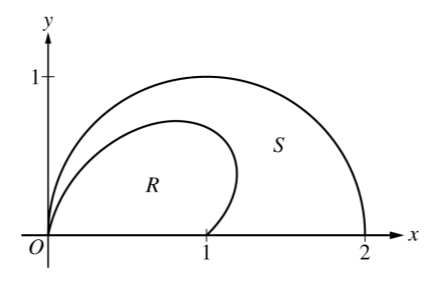
\includegraphics{./additional_materials/2017_2.png}
		\caption{\hyperref{https://apcentral.collegeboard.org/pdf/ap-calculus-bc-frq-2017.pdf}{}{}{AP Calculus BC 2017 Exam Free-Response Question 2}}
	\end{figure}

	\item The figure above show the polar curves $r=f(\theta)=1+\sin{\theta}\cos{(2\theta)}$ and $r=g(\theta)=2\cos{\theta}$ for $0 \leq \theta \leq \frac{\pi}{2}$.
		Let $R$ be the region in the first quadrant bounded by the curve $r=f(\theta)$ and the $x$-axis.
		Let $S$ be the region in the first quadrant bounded by the curve $r=f(\theta)$ the curve $r=g(\theta)$, and the $x$-axis.
		\begin{enumerate}
			\item Find the area of $R$.
			\item The ray $\theta = k$, where $0 < k < \frac{\pi}{2}$, divides $S$ into two regions of equal area.
				Write out, but do not solve, an equation involving one or more integrals whose solution gives the value of $k$.
			\item For each $\theta$, $0 \leq \theta \leq \frac{\pi}{2}$, let $w(\theta)$ be the distance between the points with polar coordinates $(f(\theta),\theta)$ and $(g(\theta),\theta)$.
				Write an expression for $w(\theta)$.
				Find $w_A$, the average value of $w(\theta)$ over the interval $0 \leq \theta \leq \frac{\pi}{2}$.
			\item Using the information given from part (c), find the value of $\theta$ for which $w(\theta)=w_A$.
				Is the function $w(\theta)$ increasing or decreasing at that value of $\theta$?
				Give a reason for your answer.
		\end{enumerate}
	
	\begin{figure}[H]
		\label{2017_3}
		\centering
		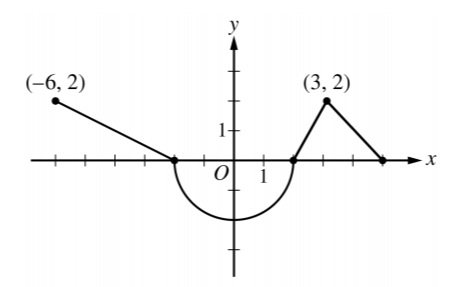
\includegraphics{./additional_materials/2017_3.png}
		\caption{\hyperref{https://apcentral.collegeboard.org/pdf/ap-calculus-bc-frq-2017.pdf}{}{}{AP Calculus BC 2017 Exam Free-Response Question 3, Graph of $f^\prime$}}
	\end{figure}
	
	\item The function $f$ is differentiable on the closed interval $[-6,5]$ and satisfies $f(-2)=7$.
		The graph of $f^\prime$, the derivative of $f$, consists of a semicircle and three line segments, as shown in the figure above.
		\begin{enumerate}
			\item Find the values of $f(-6)$ and $f(5)$.
			\item On what intervals is $f$ increasing?
				Justify your answer.
			\item Find the absolute minimum value of $f$ on the closed interval $[-6,5]$.
				Justify your answer.
			\item For each of $f^{\prime\prime}(-5)$ and $f^{\prime\prime}(3)$, find the value or explain why it doesn't exist.
		\end{enumerate}
	
	\item At time $t=0$, a boiled potato is taken from a pot on a stove and left to cool in a kitchen.
		The internal temperature of the potato is 91 degrees Celsius ($^\circ C$) at time $t=0$, and the internal temperature of the potato is greater than $27^\circ C$ for all time $t > 0$.
		The internal temperature of the potato at time $t$ minutes can be modeled by a function $H$ that satisfies the differential equation $\dd{H}{t} = -\frac{1}{4}(H-27)$, where $H(t)$ is measured in degrees Celsius and $H(0)=91$.
		\begin{enumerate}
			\item Write an equation for the line tangent to the graph of $H$ at $t=0$.
				Use this equation to approximate the internal temperature of the potato at time $t=3$.
			\item Use $\dd{^2H}{t^2}$ to determine whether your answer in part (a) is an underestimate or overestimate of the internal temperature of the potato at time $t=3$.
			\item For $t<10$, an alternate model for the internal temperature of the potato at time $t$ minutes is the function $G$ that satisfies the differential equation $\dd{G}{t} = -(G-27)^{2/3}$, where $G(t)$ is measured in degrees Celsius and $G(0)=91$.
				Based on this model, what is the internal temperature of the potato at time $t=3$?
		\end{enumerate}
	
	\item Let $f$ be the function defined by $f(x) = \frac{3}{2x^2-7x+5}$.
		\begin{enumerate}
			\item Find the slope of the tangent line of the graph of $f$ at $x=3$.
			\item Find the $x$-coordinate of each critical point of $f$ in the interval $1 < x < 2.5$.
				Classify each critical point as the location of a relative minimum, a relative maximum, or neither.
				Justify your answer.
			\item Using the identity that $\frac{3}{2x^2-7x+5} = \frac{2}{2x-5} - \frac{1}{x-1}$, evaluate $\int_{5}^{\infty}{f(x)\d{x}}$ or show that the integral diverges.
			\item Determine whether the series $\sum_{n=5}^{\infty}{\frac{3}{2n^2-7n+5}}$ converges or diverges.
				State the conditions of the test used for determining convergence or divergence.
		\end{enumerate}
	
	\begin{align*}
		f(0) &= 0 \\
		f^\prime(0) &= 1 \\
		f^{(n+1)}(0) &= -n\cdot f^{(n)}(0) \text{ for all } n \geq 1
	\end{align*}
	
	\item A function $f$ has derivatives of all order for $-1 < x < 1$.
		The derivatives of $f$ satisfy the conditions above.
		The Maclaurin Series for $f$ converges to $f(x)$ for $\abs{x} < 1$.
		\begin{enumerate}
			\item Show that the first four non-zero terms of the Maclaurin series for $f$ are $x - \frac{x^2}{2} + \frac{x^3}{3} - \frac{x^4}{4}$, and write the general term for the Maclaurin series for $f$.
			\item Determine whether the Maclaurin series described in part (a) converges absolutely, converges conditionally, or diverges at $x=1$.
				Explain your reasoning.
			\item Write the first four nonzero terms and the general term for the Maclaurin series for $g(x) = \int_{0}^{x}{f(t)\d{t}}$.
			\item Let $P_n\left(\frac{1}{2}\right)$ represent the $n$th degree Taylor polynomial for $g$ about $x=0$ and evaluated at $x=\frac{1}{2}$, where $g$ is the function defined in part (c).
				Use the alternating series error bound to show that
				\begin{equation*}
					\biggr\lvert P_4\left(\frac{1}{2}\right) - g\left(\frac{1}{2}\right) \biggr\rvert < \frac{1}{500}.
				\end{equation*}
		\end{enumerate}
	
\end{enumerate}
\subsection{2017 Free-Response Answers}

\begin{enumerate}
	\item \begin{enumerate}
		\item Using a left Riemann sum,
			\begin{equation*}
				\int_{0}^{10}{A(h)\d{h}} \approx (2-0)50.3 + (5-2)14.4 + (10-5)6.5 = 100.6 + 43.2 + 32.5 = 176.3.
 			\end{equation*}
 			So, we approximate that the volume of the tank is 176.3 cubic feet.
 		\item Since we are given that the function is decreasing over the interval, a left Riemann sum will overestimate the volume.
 		\item Integrating $f$ from $h=0$ to $h=10$,
 			\begin{equation*}
 				\int_{0}^{10}{\frac{50.3}{e^{0.2h}+h}\d{h}} \approx 101.325.
 			\end{equation*}
 			So, the volume of the tank given by $f$ is 101.325 cubic feet.
 		\item We know from (c) that
 			\begin{equation*}
 				V(h) = \int_{0}^{h}{f(x)\d{x}}.
 			\end{equation*}
 			Differentiating with respect to $t$, and applying the chain rule,
 			\begin{equation*}
 				\dd{V}{t} = f(h)\cdot\dd{h}{t}.
 			\end{equation*}
 			Plugging in $h=5$ and $\dd{h}{t}=0.26$,
 			\begin{equation*}
 				\dd{V}{t}_{h=5} = \frac{50.3}{e^1 + 5}\cdot 0.26 \approx 1.694.
 			\end{equation*}
 			So, when $h=5$ feet, the volume is changing at a rate of 1.694 cubic feet per minute.
	\end{enumerate}

	\item \begin{enumerate}
		\item Finding the area enclosed by $f$ from $\theta=0$ to $\theta=\pi/2$,
			\begin{equation*}
				A = \frac{1}{2}\int_{0}^{\pi/2}{\left(1+\sin{\theta}\cos{(2\theta)}\right)^2d\theta} \approx 0.648.
			\end{equation*}
		\item Our ray $\theta=k$ will represent a lower bound in one integral and an upper bound in the other.
			Finding equal areas between $g$ and $f$,
			\begin{equation*}
				\frac{1}{2}\int_{0}^{k}{\left(\left(2\cos{\theta}\right)^2-\left(1+\sin{\theta}\cos{(2\theta)}\right)^2\right)d\theta} = \frac{1}{2}\int_{k}^{\pi/2}{\left(\left(2\cos{\theta}\right)^2-\left(1+\sin{\theta}\cos{(2\theta)}\right)^2\right)d\theta}.
			\end{equation*}
		\item
			Since both $f$ and $g$ are polar functions evaluated at $\theta$, the distance between then will simply be the difference in their radii.
			\begin{equation*}
				w(\theta) = g(\theta) - f(\theta).
			\end{equation*} 
			Finding the average of $w$,
			\begin{equation*}
				w_A = \frac{1}{\pi/2 - 0}\int_{0}^{\pi/2}{(2\cos{\theta}-(1+\sin{\theta}\cos{(2\theta)}))\d{\theta}} \approx 0.485.
			\end{equation*}
		\item Solving $w(\theta) = w_A$,
			\begin{equation*}
				2\cos{\theta}-(1+\sin{\theta}\cos{(2\theta)}) = 0.485 \implies \theta \approx 0.518.
			\end{equation*}
			Evaluating $w^\prime(0.518)$,
			\begin{equation*}
				w^\prime(0.518) \approx -0.581.
			\end{equation*}
			So, $w$ is decreasing at this value.
	\end{enumerate}

	\item \begin{enumerate}
		\item Applying the Fundamental Theorem of Calculus,
			\begin{align*}
				\int_{-6}^{-2}{f^\prime(x)\d{x}} &= f(-2) - f(-6) = 7 - f(-6) = 4 \implies f(-6) = 3 \\
				\int_{-2}^{5}{f^\prime(x)\d{x}} &= f(5) - f(-2) = f(5) - 7 = -2\pi + 3 \implies f(5) = 10 - 2\pi.
			\end{align*}
		\item $f$ is increasing when its derivative is positive.
			Looking at the graph of $f^\prime$, we see it is positive on $[-6,2) \cup (2,5)$.
			So, $f$ is increasing on $[-6,2] \cup [2,5]$\footnote{I personally don't think $f$ is ``increasing" on the open endpoints where the derivative is 0. I think it's neither increasing nor decreasing. However, the test writers and graders feel differently, and I can't say their view is necessarily wrong.}.
		\item We see that the critical points of $f^\prime$ are $x=-2$ and $x=2$.
			A minimum can occur at a left/right endpoint that will/was decreasing.
			So, the two points we need to consider for the absolute minimum are $x=-6$ and $x=2$.
			We know from (a) that $f(-6)=3$.
			Applying the Fundamental Theorem of Calculus again,
			\begin{equation*}
				\int_{-2}^{2}{f^\prime(x)\d{x}} = f(2) - f(-2) = f(2) - 7 = 2\pi \implies f(2) = 7-2\pi.
			\end{equation*}
			Since  $7-2\pi < 3$, the absolute minimum of $f$ is at $x=2$.
		\item $f^{\prime\prime}(-5) = -\frac{1}{2}$ because $f$ is continuous at -5, and the left and right hand limits are both the slope of the line, which is $-\frac{1}{2}$.
			$f^{\prime\prime}(3) = \text{DNE}$.
			The left hand limit is the slope of the left hand line, which is 2, and the right hand limit is the left of the right hand line, which is -1.
			Since the limits do not agree, $f^\prime$ is not continuous, and hence not differentiable at $x=3$.
	\end{enumerate}

	\item \begin{enumerate}
		\item Writing the line in point-slope form and then converting to standard form,
			\begin{align*}
				y - y_0 &= m(t-t_0) \\
				y - H(0) &= \dd{H}{t}_{t=0}(t-0) \\
				y - 91 &= -16t \\
				y &= -16t + 91.
			\end{align*}
			Using this line to approximate $H(3)$,
			\begin{equation*}
				y = -16(3) + 91 = 43.
			\end{equation*}
			So, the tangent line at $t=0$ approximates $H(3)$ to be $43^\circ C$.
		\item Taking the derivative of $\dd{H}{t}$,
			\begin{equation*}
				\dd{^2H}{t^2} = -\frac{1}{4}.
			\end{equation*}
			Since the graph is concave down at every point, the tangent line at $t=0$ gives an overestimate of $H(3)$.
		\item This is a separable differential equation.
			\begin{align*}
				\dd{G}{t} &= -(G-27)^{2/3} \\
				\frac{\d{G}}{(G-27)^{2/3}} &= -1\d{t} \\
				\int{\frac{\d{G}}{(G-27)^{2/3}}} &= \int{-1\d{t}} \\
				3(G-27)^{1/3} &= -t + C \\
				(G-27)^{1/3} &= -t/3 + C \\
				G - 27 &= \left(-t/3 + C\right)^3 \\
				G &= \left(-t/3 + C\right)^3 + 27.
			\end{align*}
			Solving for $C$ using $G(0)=91$,
			\begin{align*}
				91 &= \left(-0/3 + C\right)^2 + 27 \\
				64 &= C^3 \\
				C &= 4.
			\end{align*}
			So, our overall solution for $G$ is
			\begin{equation*}
				G(t) = \left(4 - t/3\right)^3 + 27.
			\end{equation*}
			Evaluating at $t=3$,
			\begin{equation*}
				G(3) = \left(4 - 3/3\right)^3 + 27 = 3^3  + 27 = 54.
			\end{equation*}
			So, the internal temperature of the potato at $t=3$ minutes is $54^\circ C$.
	\end{enumerate}

	\item \begin{enumerate}
		\item Applying the quotient rule,
			\begin{equation*}
				f^\prime(x) = \frac{(2x^2-7x+5)(0)-3(4x-7)}{(2x^2-7x+5)^2} = \frac{-12x+21}{(2x^2-7x+5)^2}.
			\end{equation*}
			Evaluating at $x=3$,
			\begin{equation*}
				f^\prime(3) = \frac{-12(3)+21}{(2(3)^2-7(3)+5)^2} = -\frac{15}{(18-21+5)^2} = -\frac{15}{4}.
			\end{equation*}
		\item $f^\prime(x)=0$ only when the numerator is 0,
			\begin{equation*}
				-12x + 21 = 0 \implies x = \frac{7}{4}.
			\end{equation*}
			$f^\prime$ is negative to the left of $\frac{7}{4}$ and positive to the right of it.
			Therefore, $x=\frac{7}{4}$ is a relative maximum by the first derivative test.
		\item Evaluating the limit using the given partial fraction decomposition,
			\begin{align*}
				\int_{5}^{\infty}{f(x)\d{x}} &= \int_{5}^{\infty}{\left(\frac{2}{2x-5}-\frac{1}{x-1}\right)\d{x}} \\
				&= \ln{(2x-5)} - \ln{(x-1)} \biggr\rvert_{5}^{\infty} \\
				&= \ln{\left(\frac{2x-5}{x-1}\right)} \biggr\rvert_{5}^{\infty} \\
				&= \lim_{b\to\infty}{\ln{\left(\frac{2b-5}{b-1}\right)}} - \ln{\left(\frac{5}{4}\right)} \\
				&= \ln{2} - \ln{\left(\frac{5}{4}\right)} \\
				&= \ln{\left(\frac{8}{5}\right)}.
			\end{align*}
		\item For $n \geq 5$, $f(n)$ is positive and decreasing.
			Using our work from part (c), we know that the integral of $f$ from 5 to $\infty$ converges.
			So, by the Integral test, the series also converges.
	\end{enumerate}

	\item \begin{enumerate}
		\item Calculating the first four derivatives and the general derivative,
			\begin{align*}
				f(0) &= 0 \\
				f^\prime(0) &= 1 \\
				f^{\prime\prime}(0) &= -1\cdot f^\prime(0) = -1 \\
				f^{(3)}(0) &= -2\cdot f^{\prime\prime}(0) = 2 \\
				f^{(4)}(0) &= -3\cdot f^{(3)}(0) = -6.
				f^{(n+1)}(0) &= -n\cdot f^{(n)}(0) = (-1)^{n+1}n!.
			\end{align*}
			Applying the Maclaurin series formula,
			\begin{align*}
				P_n(x) &= \frac{f(0)}{0!} + \frac{f^\prime(0)}{1!}x + \frac{f^{\prime\prime}(0)}{2!}x^2 + \ldots + \frac{f^{(n)}(0)}{n!}x^n \\
				&= \frac{0}{1} + \frac{1}{1}x + \frac{-1}{2}x^2 + \frac{2}{6}x^3 + \frac{-6}{24}x^4 + \ldots + \frac{(-1)^{n+1}(n-1)!}{n!}x^n \\
				&= x - \frac{x^2}{2} + \frac{x^3}{3} - \frac{x^4}{4} + \ldots + (-1)^{n+1}\frac{x^n}{n}.
			\end{align*}
		\item At $x=1$, the series is
			\begin{equation*}
				\sum_{n=1}^{\infty}{(-1)^{n+1}\frac{1}{n}}.
			\end{equation*}
			This series converges by the Alternating Series test, which determines conditional converges.
			So, the series converges conditionally at $x=1$.
		\item Integrating term-by-term,
			\begin{align*}
				g(x) &= \int_{0}{x}{f(t)\d{t}} \\
				&= \int_{0}^{x}{\left(t-\frac{t^2}{2}+\frac{t^3}{3}-\frac{t^4}{4}+\ldots+(-1)^{n+1}\frac{t^n}{n}\right)\d{t}} \\
				&= \frac{t^2}{2} - \frac{t^3}{6} + \frac{t^4}{12} - \frac{t^5}{20} + \ldots + (-1)^{n+1}\frac{t^{n+1}}{n(n+1)} \biggr\rvert_{0}^{x} \\
				&= \frac{x^2}{2} - \frac{x^3}{6} + \frac{x^4}{12} - \frac{x^5}{20} + \ldots + (-1)^{n+1}\frac{x^{n+1}}{n(n+1)}.
			\end{align*}
		\item The Alternating Series Estimation Theorem tells us that the upper bound for the error is the absolute value of the first not included term.
			For $P_4$, this term is $-\frac{x^5}{20}$.
			So,
			\begin{align*}
				\biggr\lvert P_4\left(\frac{1}{2}\right) - g\left(\frac{1}{2}\right) \biggr\rvert < \biggr\lvert -\frac{\left(\frac{1}{2}\right)^5}{20} \biggr\rvert = \frac{1}{640} < \frac{1}{500}.
			\end{align*}
	\end{enumerate}

\end{enumerate}
\subsection{2016 Free-Response Questions}
Questions 1 and 2 part of the same section area are allotted 30 minutes from completion with the aid of a graphing calculator.
Questions 3 through 6 are part of the same section and area allotted 1 hour from completion without the aid of a graphing calculator.

\begin{table}[H]
	\begin{center}
		\begin{tabular}{|c||c|c|c|c|c|}
			\hline
			$t$ (hours) & 0 & 1 & 3 & 6 & 8 \\
			\hline
			$R(t)$ (liters / hour) & 1340 & 1190 & 950 & 740 & 700 \\
			\hline
		\end{tabular}
	\end{center}
\end{table}

\begin{enumerate}
	\item Water is pumped into a tank at a rate modeled by $W(t)=2000e^{-t^2/20}$ liters per hour for $0 \leq t \leq 8$, where $t$ is measured in hours.
	Water is removed from the tank at a rate modeled by $R(t)$ liters per hour, where $R$ is differentiable and decreasing on $0 \leq t \leq 8$.
	Selected values of $R(t)$ are shown in the table above.
	At time $t=0$, there are 50000 liters of water in the tank.
	\begin{enumerate}
		\item Estimate $R^\prime(2)$.
		Show the work that leads to your answer.
		Indicate units of measure.
		\item Use a left Riemann sum with the four subintervals indicated by the table to estimate the total amount of water removed from the tank during the 8 hours.
		Is this an over estimate or underestimate of the total amount of water removed?
		Give a reason for your answer.
		\item Use your answer from part (b) to find an estimate for the total amount of water in the tank, to the nearest liters, at the end of the 8 hours.
		\item For $0 \leq t \leq 8$, is there a time $t$ when the rate at which the water is pumped into the tank is the same rate as the rate at which water is removed from the tank?
		Explain why or why not.
	\end{enumerate}

	\begin{figure}[H]
		\label{2016_2}
		\centering
		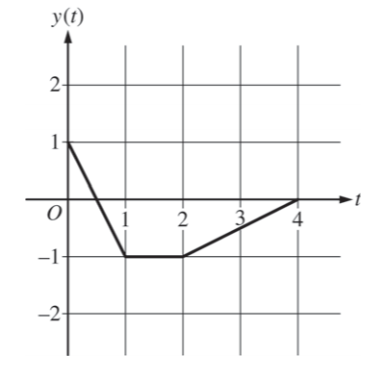
\includegraphics{./additional_materials/2016_2.png}
		\caption{\hyperref{https://secure-media.collegeboard.org/digitalServices/pdf/ap/ap16\_frq\_calculus\_bc.pdf}{}{}{AP Calculus BC 2016 Exam Free-Response Question 2}}
	\end{figure}
	
	\item At time $t$, the position of a particle moving in the $xy$-plane is given by the parametric functions $(x(t),y(t))$, where $\dd{x}{t} = t^2 + \sin{(3t^2)}$.
		The graph of $y$ consisting of three line segments, is shown in the figure above.
		At $t=0$, the particle is at position $(5,1)$.
		\begin{enumerate}
			\item Find the position of the particle at $t=3$.
			\item Find the slope of the line tangent to the part of the particle at $t=3$.
			\item Find the speed of the particle at $t=3$.
			\item Find the total distance traveled by the particle from $t=0$ to $t=2$.
		\end{enumerate}
	
	\begin{figure}[H]
		\label{2016_3}
		\centering
		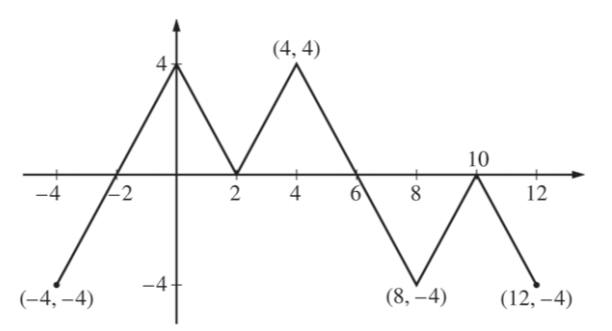
\includegraphics{./additional_materials/2016_3.png}
		\caption{\hyperref{https://secure-media.collegeboard.org/digitalServices/pdf/ap/ap16\_frq\_calculus\_bc.pdf}{}{}{AP Calculus BC 2016 Exam Free-Response Question 3, Graph of $f$}}
	\end{figure}
	
	\item The figure above shows the graph of the piecewise-linear function $f$.
		For $-4 \leq x \leq 12$, the function $g$ is defined by $g(x)=\int_{2}^{x}{f(t)\d{t}}$.
		\begin{enumerate}
			\item Does $g$ have a relative minimum, a relative maximum, or neither at $x=10$?
				Justify your answer.
			\item Does the graph of $g$ have a point of inflection at $x=4$?
				Justify your answer.
			\item Find the absolute minimum value and the absolute maximum value of $g$ on the interval $-4 \leq x \leq 12$.
				Justify your answers.
			\item For $-4 \leq x \leq 12$, find all intervals for which $g(x) \leq 0$.
		\end{enumerate}
	
	\item Consider the differential equation $\dd{y}{x} = x^2 - \frac{1}{2}y$.
		\begin{enumerate}
			\item Find $\dd{^2y}{x^2}$ in terms of $x$ and $y$.
			\item Let $y=f(x)$ be the particular solution to the given differential equation whose graph passes through the point $(-2,8)$.
				Does the graph of $f$ have a relative minimum, a relative maximum, or neither at the point $(-2,8)$?
				Justify your answer.
			\item Let $y=g(x)$ be the particular solution to the given differential equation with $g(-1)=2$.
				Find $\lim_{x\to -1}{\left(\frac{g(x)-2}{3(x+1)^2}\right)}$.
				Show the work that leads to your answer.
			\item Let $y=h(x)$ be the particular solution to the given differential equation with $h(0)=2$.
				Use Euler's method, starting at $x=0$ with two steps of equal size, to approximate $h(1)$.
		\end{enumerate}
	
	\begin{figure}[H]
		\label{2016_5}
		\centering
		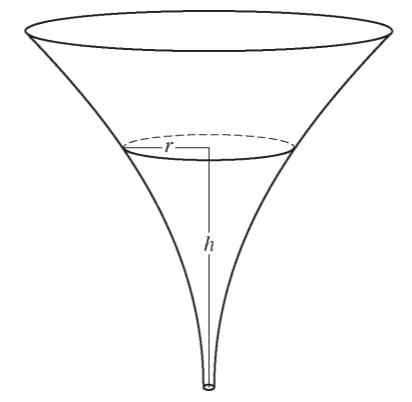
\includegraphics{./additional_materials/2016_5.png}
		\caption{\hyperref{https://secure-media.collegeboard.org/digitalServices/pdf/ap/ap16\_frq\_calculus\_bc.pdf}{}{}{AP Calculus BC 2016 Exam Free-Response Question 5}}
	\end{figure}
	
	\item The inside of a funnel of height 10 inches has circular cross sections, as shown in the figure above.
		At height $h$, the radius of the funnel is given by $r = \frac{1}{20}\left(3+h^2\right)$, where $0 \leq h \leq 10$.
		The units of $r$ and $h$ are inches.
		\begin{enumerate}
			\item Find the average value of the radius of the funnel.
			\item Find the volume of the funnel.
			\item The funnel contains liquid that is draining from the bottom.
				At the instant when the height of the liquid is $h=3$ inches, the radius of the surface of the liquid is decreasing at a rate of $\frac{1}{5}$ inch per second.
				At this instant, what is the rate of change of the height of the liquid with respect to time?
		\end{enumerate}
	
	\item The function $f$ has a Taylor series about $x=1$ that converges to $f(x)$ for all $x$ in the interval of convergence.
		It is known that $f(1)=1$, $f^\prime(1)=-\frac{1}{2}$, and the $n$th derivative of $f$ at $x=1$ is given by $f^{(n)}(1) = (-1)^{n}\frac{(n-1)!}{2^n}$ for $n \geq 2$.
		\begin{enumerate}
			\item Write the first four nonzero terms and the general term of the Taylor series for $f$ about $x=1$.
			\item The Taylor series for $f$ about $x=1$ has a radius of convergence of 2.
				Find the interval of convergence.
				Show the work that leads to your answer.
			\item The Taylor series for $f$ about $x=1$ can be used to represent $f(1.2)$ as an alternating series.
				Use the first three non-zero terms of the alternating series to approximate $f(1.2)$.
			\item Show that the approximation found in part (c) is within 0.001 of the exact value of $f(1.2)$.
		\end{enumerate}
\end{enumerate}
\subsection{2016 Free-Response Answers}

\begin{enumerate}
	\item \begin{enumerate}
		\item We can approximate $R^\prime(2)$ as the tangent slope between 1 and 3.
			\begin{equation*}
				R^\prime(2) \approx \frac{R(3)-R(1)}{3-1} = \frac{950-1190}{2} = -120.
			\end{equation*}
			So, we estimate $R^\prime(3)$ to be -120 liters/hour$^2$.
		\item Using a left Riemann sum using the values in the table,
			\begin{equation*}
				\int_{0}^{8}{R(t)\d{t}} \approx (1-0)1340 + (3-1)1190 + (6-3)950 + (8-6)740 = 1340 + 2380 + 2850 + 1480 = 8050.
			\end{equation*}
			So, the left Riemann sum approximates the total water removed to be 8050 liters.
		\item Using our answer from part (b) and integrating, we can find the total amount of water added or removed.
			\begin{equation*}
				\Delta \text{Water} = -8050 + \int_{0}{8}{2000e^{-t^2/20}\d{t}} \approx -214.
			\end{equation*}
			Since we know there is 50000 liters of water at $t=0$, we can add the net change to find the amount of water at $t=8$.
			\begin{equation*}
				\text{Water}_8 = \text{Water}_0 + \Delta \text{Water} = 50000 - 214 = 49768.
			\end{equation*}
			So, to the nearest liter, we approximate the amount of water in the tank at $t=8$ to be 49768 liters.
		\item At $t=0$, $W(0) = 2000 > R(0) = 1340$, so $W(0)-R(0) > 0$.
			At $t=8$, $W(8) = 81.52 < R(8) = 700$, so $W(8)-R(8) < 0$.
			Since both $W$ and $R$ are continuous, so is $W - R$.
			So, by the Intermediate Value Theorem, there is some $0 < t < 8$ such that $W(t)-R(t)=0$, or $W(t)=R(t)$.
	\end{enumerate}

	\item \begin{enumerate}
		\item We can apply the Fundamental Theorem of Calculus to find $x(3)$.
			\begin{equation*}
				\int_{0}^{3}{\dd{x}{t}\d{t}} = x(3) - x(0) = x(3) - 5 = 9.377 \implies x(3) = 14.377.
			\end{equation*}
			Looking at the graph, we see that $y(3)=-\frac{1}{2}$.
			So, at $t=3$, the particle's position is $\left(14.377, -0.5\right)$.
		\item Looking at the graph, we see that $y^\prime(3) = \frac{1}{2}$.
			Evaluating $\dd{x}{t}$ at $t=3$, we see that $x^\prime(3) = 9+\sin{27}$.
			So,
			\begin{equation*}
				\dd{y}{x} = \frac{\dd{y}{t}}{\dd{x}{t}} = \frac{\frac{1}{2}}{9+\sin{27}} \approx 0.0502.
			\end{equation*}
		\item Using our formula for parametric speed,
			\begin{equation*}
				s = \sqrt{(x^\prime(t))^2 + (y^\prime(t))^2} = \sqrt{\left(\frac{1}{2}\right)^2 + \left(9+\sin{27}\right)^2} \approx 9.969.
			\end{equation*}
		\item Starting with the formula for parametric arc length and splitting the integral into two peices,
			\begin{align*}
				\int_{0}^{2}{\sqrt{\left(y^\prime(t)\right)^2+\left(x^\prime(t)\right)^2}\d{t}} &= \int_{0}^{1}{\sqrt{(-2)^2+(t^2+\sin{(3t^2)})^2}\d{t}} + \int_{1}^{2}{\sqrt{(0)^2+(t^2+\sin{(3t^2)})^2}\d{t}} \\
				&\approx 2.237 + 2.112 \\
				&= 4.439.
			\end{align*}
	\end{enumerate}

	\item \begin{enumerate}
		\item Since we know by the Fundamental Theorem of Calculus that $f$ is the derivative of $g$, $g$ has critical points where $f$ is 0.
			$x=10$ is one such critical point.
			Both to the left and right of $x=10$, $f$ is negative.
			So, although $x=10$ is a critical point, it is neither a relative minimum or relative maximum of $g$ because $g$ is decreasing both left and right of $x=10$.
		\item Inflection points occur when the second derivative changes sign.
			Since $f$ is the derivative of $g$, inflection points of $g$ occur when the derivative of $f$ changes sign.
			To the left of $x=4$, the derivative of $f$ is positive.
			To the right of $x=4$, the derivative of $f$ is negative.
			So, $x=4$ is indeed an inflection point for $g$.
		\item $g$ has critical points where $f$ is 0, which is at $x=-2$, $x=2$, $x=6$, and $x=10$.
			Of these, $x=2$ and $x=10$ do not change sign, so they cannot be absolute extrema.
			Evaluating the remaining critical points and the endpoints using the geometry of the graph of $f$,
			\begin{align*}
				g(-4) &= -4 \\
				g(-2) &= -8 \\
				g(6) &= 8 \\
				g(12) &= -4.
			\end{align*}
			So, the absolute minimum of $g$ is at $x=-2$, and the absolute maximum of $g$ is at $x=6$.
		\item To the left $x=2$, $g(x)$ is negative whenever there is more area between $f$ and the $x$-axis above the $x$-axis than below.
			So, all points $[-4,2]$ have $g(x) \leq 0$.
			To the left of $x=2$, the opposite is true.
			So, all points $[10,12]$ have $g(x) \leq 0$.
			Putting these two results together, $g(x) \leq 0$ on $[-4,2] \cup [10,12]$. 
	\end{enumerate}

	\item \begin{enumerate}
		\item Implicitly differentiating,
			\begin{equation*}
				\d{^2y}{x^2} = 2x - \frac{1}{2}\dd{y}{x} = 2x - \frac{1}{2}\left(x^2 - \frac{1}{2}y\right).
			\end{equation*}
		\item Since we have expression for the first and second derivatives, it makes the most sense to apply a second derivative test.
			First, checking that $(-2,8)$ is indeed a critical point,
			\begin{equation*}
				\dd{y}{x}_{(-2,8)} = (-2)^2 - \frac{1}{2}(8) = 0.
			\end{equation*}
			Next, evaluating the second derivative,
			\begin{equation*}
				\dd{^2y}{x^2}_{(-2,8)} = 2(-2) - \frac{1}{2}\left((-2)^2 - \frac{1}{2}(8)\right) = -4 - 0 = -4.
			\end{equation*}
			Since the second derivative is negative at this critical point, the second derivative test tells us that this is a relative maximum.
		\item Since we know that $g(-1)=2$, both the numerator and denominator of the limit are in an indeterminate form of 0/0.
			So, we can apply L'H\^{o}pital's Rule.
			\begin{equation*}
				\lim_{x\to -1}{\left(\frac{g(x)-2}{3(x+1)^2}\right)} = \lim_{x\to-1}\left(\frac{g^\prime(x)}{6(x+1)}\right).
			\end{equation*}
			Using the given differential equation, we can see that at $(-1,2)$, $g^\prime(-1)=0$.
			So again we have an indeterminate form of 0/0 and can apply L'H\^{o}pital's Rule.
			\begin{equation*}
				\lim_{x\to-1}\left(\frac{g^\prime(x)}{6(x+1)}\right) = \lim_{x\to -1}{\frac{g^{\prime\prime}(x)}{6}}.
			\end{equation*}
			Using our answer from part (b), we know that at $(-1,2)$, $g^{\prime\prime}(-1) = -2$.
			So,
			\begin{equation*}
				\lim_{x\to -1}{\frac{g^{\prime\prime}(x)}{6}} = \frac{-2}{6} = -\frac{1}{3}.
			\end{equation*}
		\item Applying two iterations of Euler's method starting at $(0,2)$ with $\Delta x = \frac{1}{2}$,
			\begin{table}[H]
				\begin{center}
					\begin{tabular}{|c|c|c|c|c|}
						\hline
						$(x,y)$ & $\dd{y}{x}$ & $\Delta x$ & $\Delta y = \Delta x\dd{y}{x}$ & $(x+\Delta x, y+\Delta y)$ \\
						\hline
						$(0,2)$ & $-1$ & $\frac{1}{2}$ & $-\frac{1}{2}$ & $(\frac{1}{2},\frac{3}{2})$ \\
						\hline
						$(\frac{1}{2},\frac{3}{2})$ & $-\frac{1}{2}$ & $\frac{1}{2}$ & $-\frac{1}{4}$ & $(1,\frac{5}{4})$ \\
						\hline
					\end{tabular}
				\end{center}
			\end{table}
			So, our application of Euler's method approximates $h(1)$ to be 5/4.
	\end{enumerate}

	\item \begin{enumerate}
		\item Applying the formula for average value,
			\begin{equation*}
				\frac{1}{10-0}\int_{0}^{10}{\frac{1}{20}\left(3+h^2\right)\d{h}} = \frac{1}{200}\left(3h+\frac{h^3}{3}\right) = \frac{109}{60}.
			\end{equation*}
			So, the average radius of the funnel is $\frac{109}{60}$ inches.
		\item Applying the volume formula for a solid of revolution,
			\begin{align*}
				V &= \pi\int_{0}^{10}{\left(\frac{1}{20}\left(3+h^2\right)\right)\d{h}} \\
				&= \frac{\pi}{400}\left(\frac{h^5}{5}+2h^3+9h\right)\biggr\rvert_0^{10} \\
				&= \frac{\pi}{400}\left(20000+2000+90\right) \\
				&= \frac{2209\pi}{40}.
			\end{align*}
		\item Applying the chain rule,
			\begin{align*}
				\dd{r}{t} &= \dd{r}{h}\dd{h}{t} \\
				&= \frac{1}{10}h\dd{h}{t}.
			\end{align*}
			Solving with the information given,
			\begin{equation*}
				-\frac{1}{5} = \frac{1}{10}(3)\dd{h}{t} \implies \dd{h}{t} = -\frac{2}{3}.
			\end{equation*}
			So, at this instant, the height of the liquid is decreasing at 2/3 inches per second.
	\end{enumerate}

	\item \begin{enumerate}
		\item Finding several derivatives at $x=1$,
			\begin{align*}
				f(1) &= 1 \\
				f^\prime(1) &= -\frac{1}{2} \\
				f^{\prime\prime}(1) &= \frac{1}{4} \\
				f^{(3)}(1) &= -\frac{1}{4}.
			\end{align*}
			Applying the Taylor Series formula centered at $x=1$,
			\begin{equation*}
				f(x) = 1 - \frac{1}{2}(x-1) + \frac{1}{8}(x-1)^2 - \frac{1}{24}(x-1)^3 + \ldots + (-1)^n\frac{1}{n2^n}(x-1)^n.
			\end{equation*}
		\item Since we know that the series is centered at $x=1$ and the radius of convergence is 2, we know the series converges on $(-1,3)$ and need to check the endpoints.
			When $x=-1$,
			\begin{equation*}
				\sum_{n=1}^{\infty}{(-1)^n\frac{1}{n2^n}(-1-1)^n} = \sum_{n=1}^{\infty}{\frac{1}{n}}
			\end{equation*}
			diverges by the P-Test.
			When $x=3$,
			\begin{equation*}
				\sum_{n=1}^{\infty}{(-1)^n\frac{1}{n2^n}(3-1)^n} = \sum_{n=1}^{\infty}{(-1)^n\frac{1}{n}}
			\end{equation*}
			converges by the Alternating Series Test.
			So, the invterval of convergence is $(-1,3]$.
		\item Using the first three terms of our series from part (a) with $x=1.2$,
			\begin{equation*}
				f(1.2) \approx 1 - \frac{1}{2}(1.2-1) + \frac{1}{8}(1.2-1)^2 = 1 - \frac{1}{10} + \frac{1}{200} = 0.905.
			\end{equation*}
		\item Since this series is alternating, we can apply the Alternating Series Estimation Theorem.
			\begin{equation*}
				\abs{f(1.2)-P_2(1.2)} \leq \abs{\frac{-1}{2^3\cdot 3} (.2)^3 } = \frac{1}{3000} \leq 0.001.
			\end{equation*}
			So, by the Alternating Series Estimation Theorem, the error is certainly at most 0.001.
	\end{enumerate}
\end{enumerate}

% Online Resources
\section{Online Resources}
\noindent
Below is a list of other useful resources for learning differential equations. Most are freely accessible online.
\begin{itemize}
	\item
		\href{http://tutorial.math.lamar.edu/Classes/DE/DE.aspx}{Paul's Online Notes} -- Goes deeper than this text and has additional practices problems.
	\item
		\href{https://www.khanacademy.org/math/differential-equations}{Khan Academy} -- Video lectures and practice problems.
	\item
		\href{https://www.youtube.com/playlist?list=PLD4B0062CA82D73FB}{PatrickJMT} -- YouTube series focused mostly on solving example problems.
	\item
		\href{https://ocw.mit.edu/courses/mathematics/18-03sc-differential-equations-fall-2011/}{MIT OCW 18.03SC} -- Complete series of lectures, recitations, assignments, practice problems, lecture notes, and exams needed for independent study.
	\item
		\href{https://www.math.ust.hk/~machas/differential-equations.pdf}{Jeffery R. Chasnov: Differential Equations} -- Online textbook from the Hong Kong University of Science and Technology. Adapted from Coursera's Differential Equations for Engineers.
\end{itemize}
% Contributors
\section{Contributors}
Special thanks to everyone who made contributions to this project on \href{https://github.com/wmboyles/Math-Summaries}{Github}.
They are listed in order of number of commits as \texttt{name (GitHub username)}.

\begin{center}
    \begin{tabular}{ c c c }
    	William Boyles (\href{https://api.github.com/users/wmboyles}{wmboyles}) & Ashwin M  (\href{https://api.github.com/users/Suzukazole}{Suzukazole}) & aneziac (\href{https://api.github.com/users/aneziac}{aneziac}) \\
		Aditya Dev (\href{https://api.github.com/users/dev-aditya}{dev-aditya}) & Calvin McPhail-Snyder (\href{https://api.github.com/users/esselltwo}{esselltwo}) & Robert Washbourne (\href{https://api.github.com/users/rawsh}{rawsh}) \\
	\end{tabular}
\end{center}
\fi	% Additional Resources
		
		% Other possible sections
			% "Real World" Applications
				% Viral spread / logistic function
				% Circuits
			% Numerical methods
				% Euler's method
				% Picard's method
				% Taylor series
				% Ranga Kutta
			% Chaos
				% Period doubling
				% Strange attractor
		% Notes / TODOS
			% I don't put periods after equations that are in the middle of a sentence. Apparently this is a mortal sin. I'm pretty sure I obeyed capitalization rules, so you can see when a new sentence starts after an equation because the new sentence will begin with a capital letter.
	\backmatter
\end{document}